\documentclass[conference]{IEEEtran}
\IEEEoverridecommandlockouts
% The preceding line is only needed to identify funding in the first footnote. If that is unneeded, please comment it out.
\usepackage{cite}
\usepackage{amsmath,amssymb,amsfonts}
\usepackage{algorithmic}
\usepackage{graphicx}
\usepackage{textcomp}
\usepackage{xcolor}
\def\BibTeX{{\rm B\kern-.05em{\sc i\kern-.025em b}\kern-.08em
    T\kern-.1667em\lower.7ex\hbox{E}\kern-.125emX}}
\begin{document}

\title{CENG 466 - Image Processing THE4 Report} \\
\author{
\IEEEauthorblockN{Muhammed Enes izgi}
\IEEEauthorblockA{\textit{Computer Engineering} \\
\textit{METU}\\
Ankara, Turkey \\
enes.izgi@metu.edu.tr}
\and
\IEEEauthorblockN{Emre Berk Kaya}
\IEEEauthorblockA{\textit{Computer Engineering} \\
\textit{METU}\\
Ankara, Turkey \\
emre.kaya\_03@metu.edu.tr}
}

\maketitle

\section{Introduction}
This document explains the methods used in fourth homework of Image Processing course.

\section{Object Detection}

In this part, we are using thresholding and morphological methodologies to detect flowers. First, we are converting our image into grayscale. Now, we need to find a threshold value and then use that threshold value to mask our image. \\

Firstly, we tried to use Otsu thresholding to dynamically determine the threshold value. Otsu thresholding gives us good results but we decided to use a threshold value as a parameter because we can fine-tune our algorithm for individual images better this way.

After masking our image with the threshold value, for A1.png, we had an image like this: \\ \\
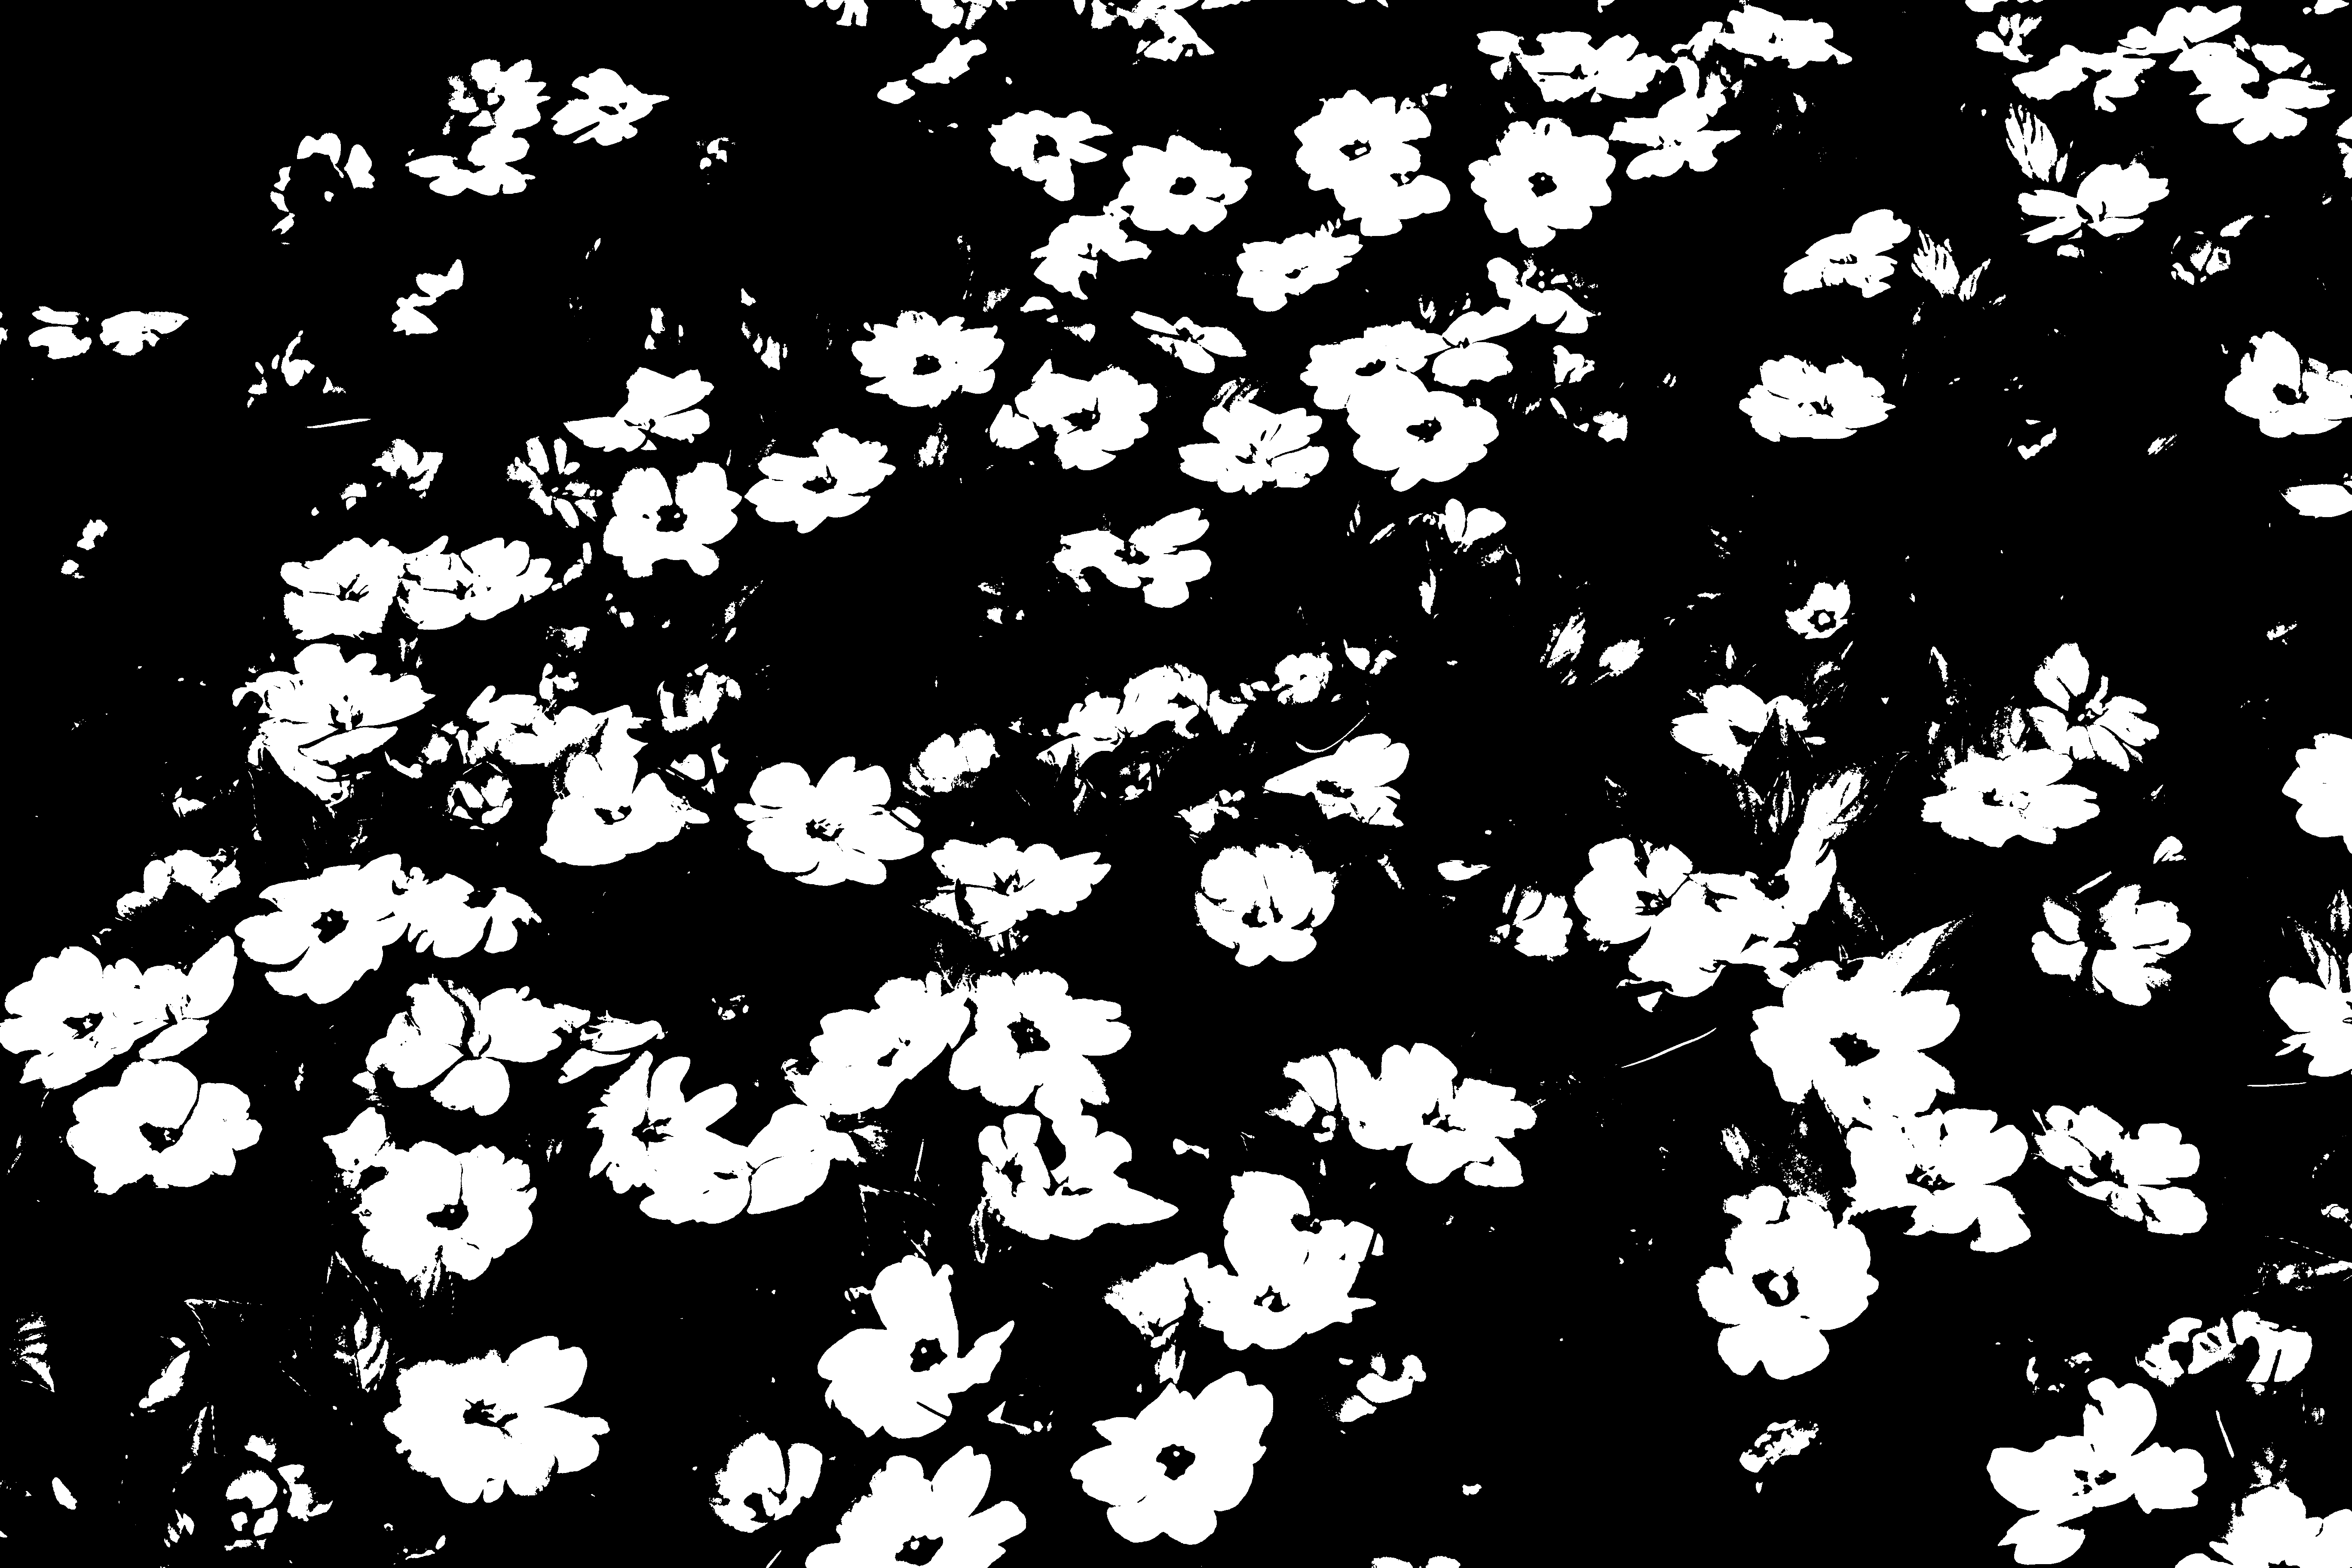
\includegraphics[scale=0.04]{A1_thresh.png} \\ \\
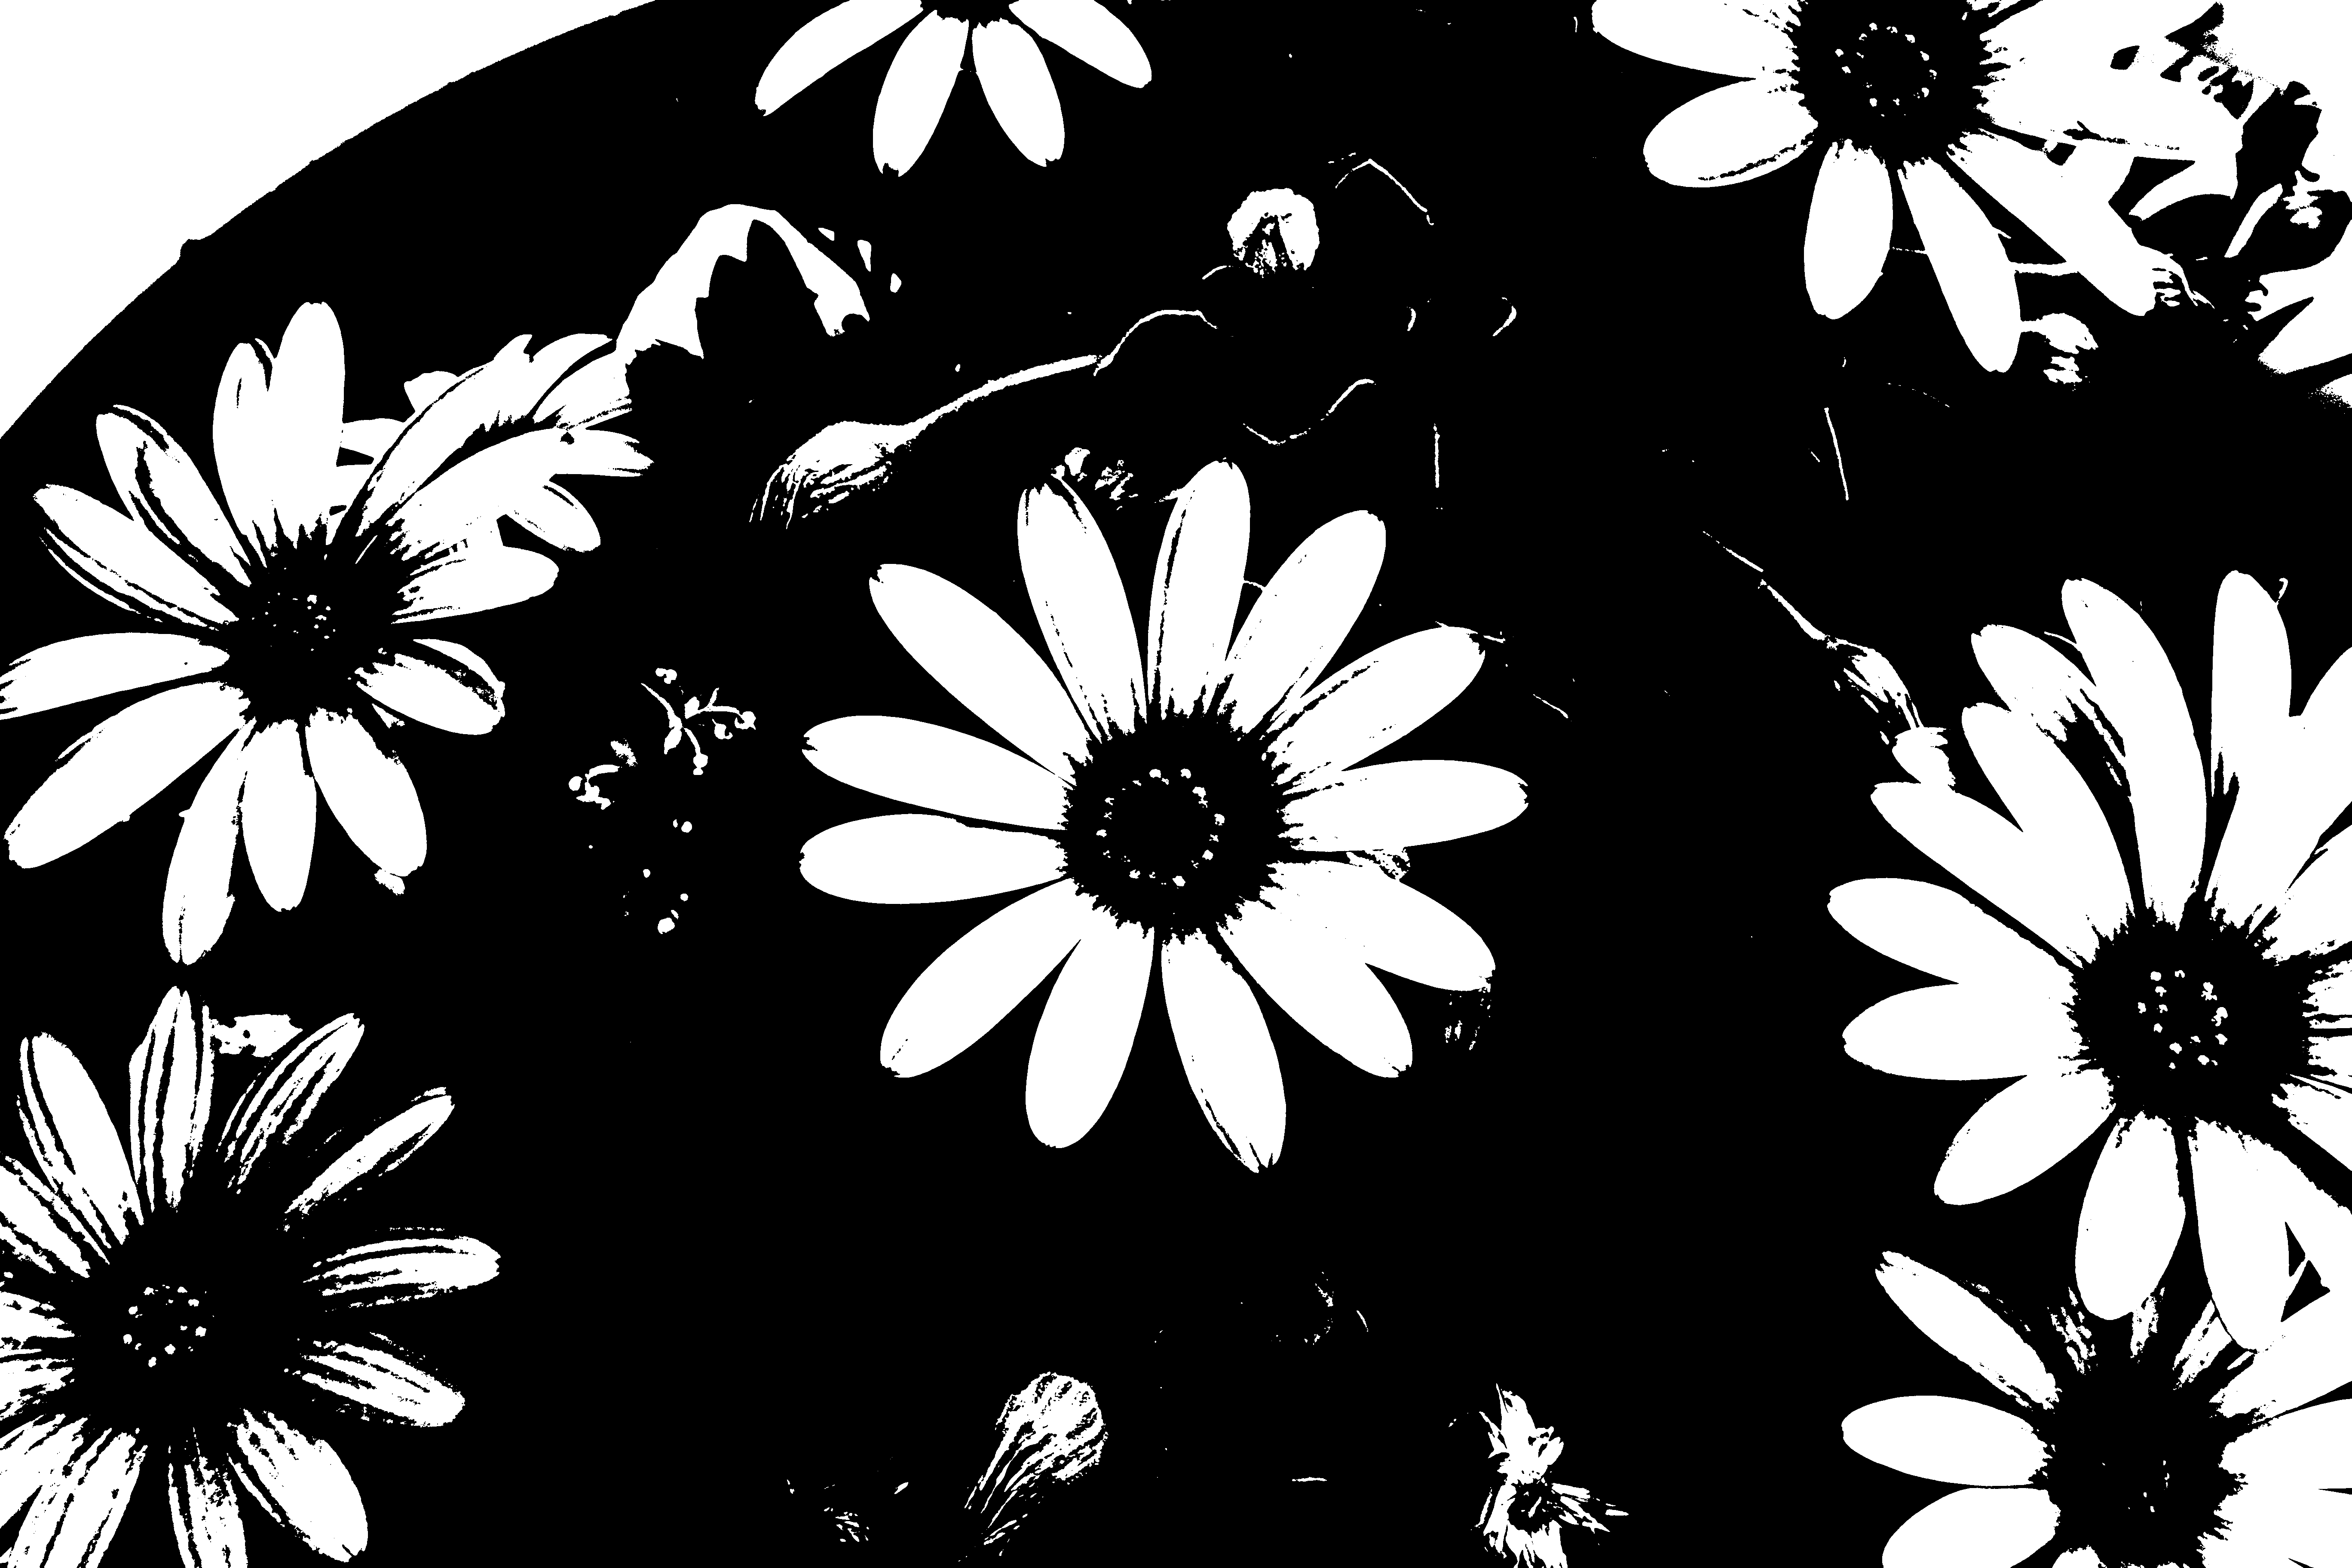
\includegraphics[scale=0.04]{A2_thresh.png} \\ \\
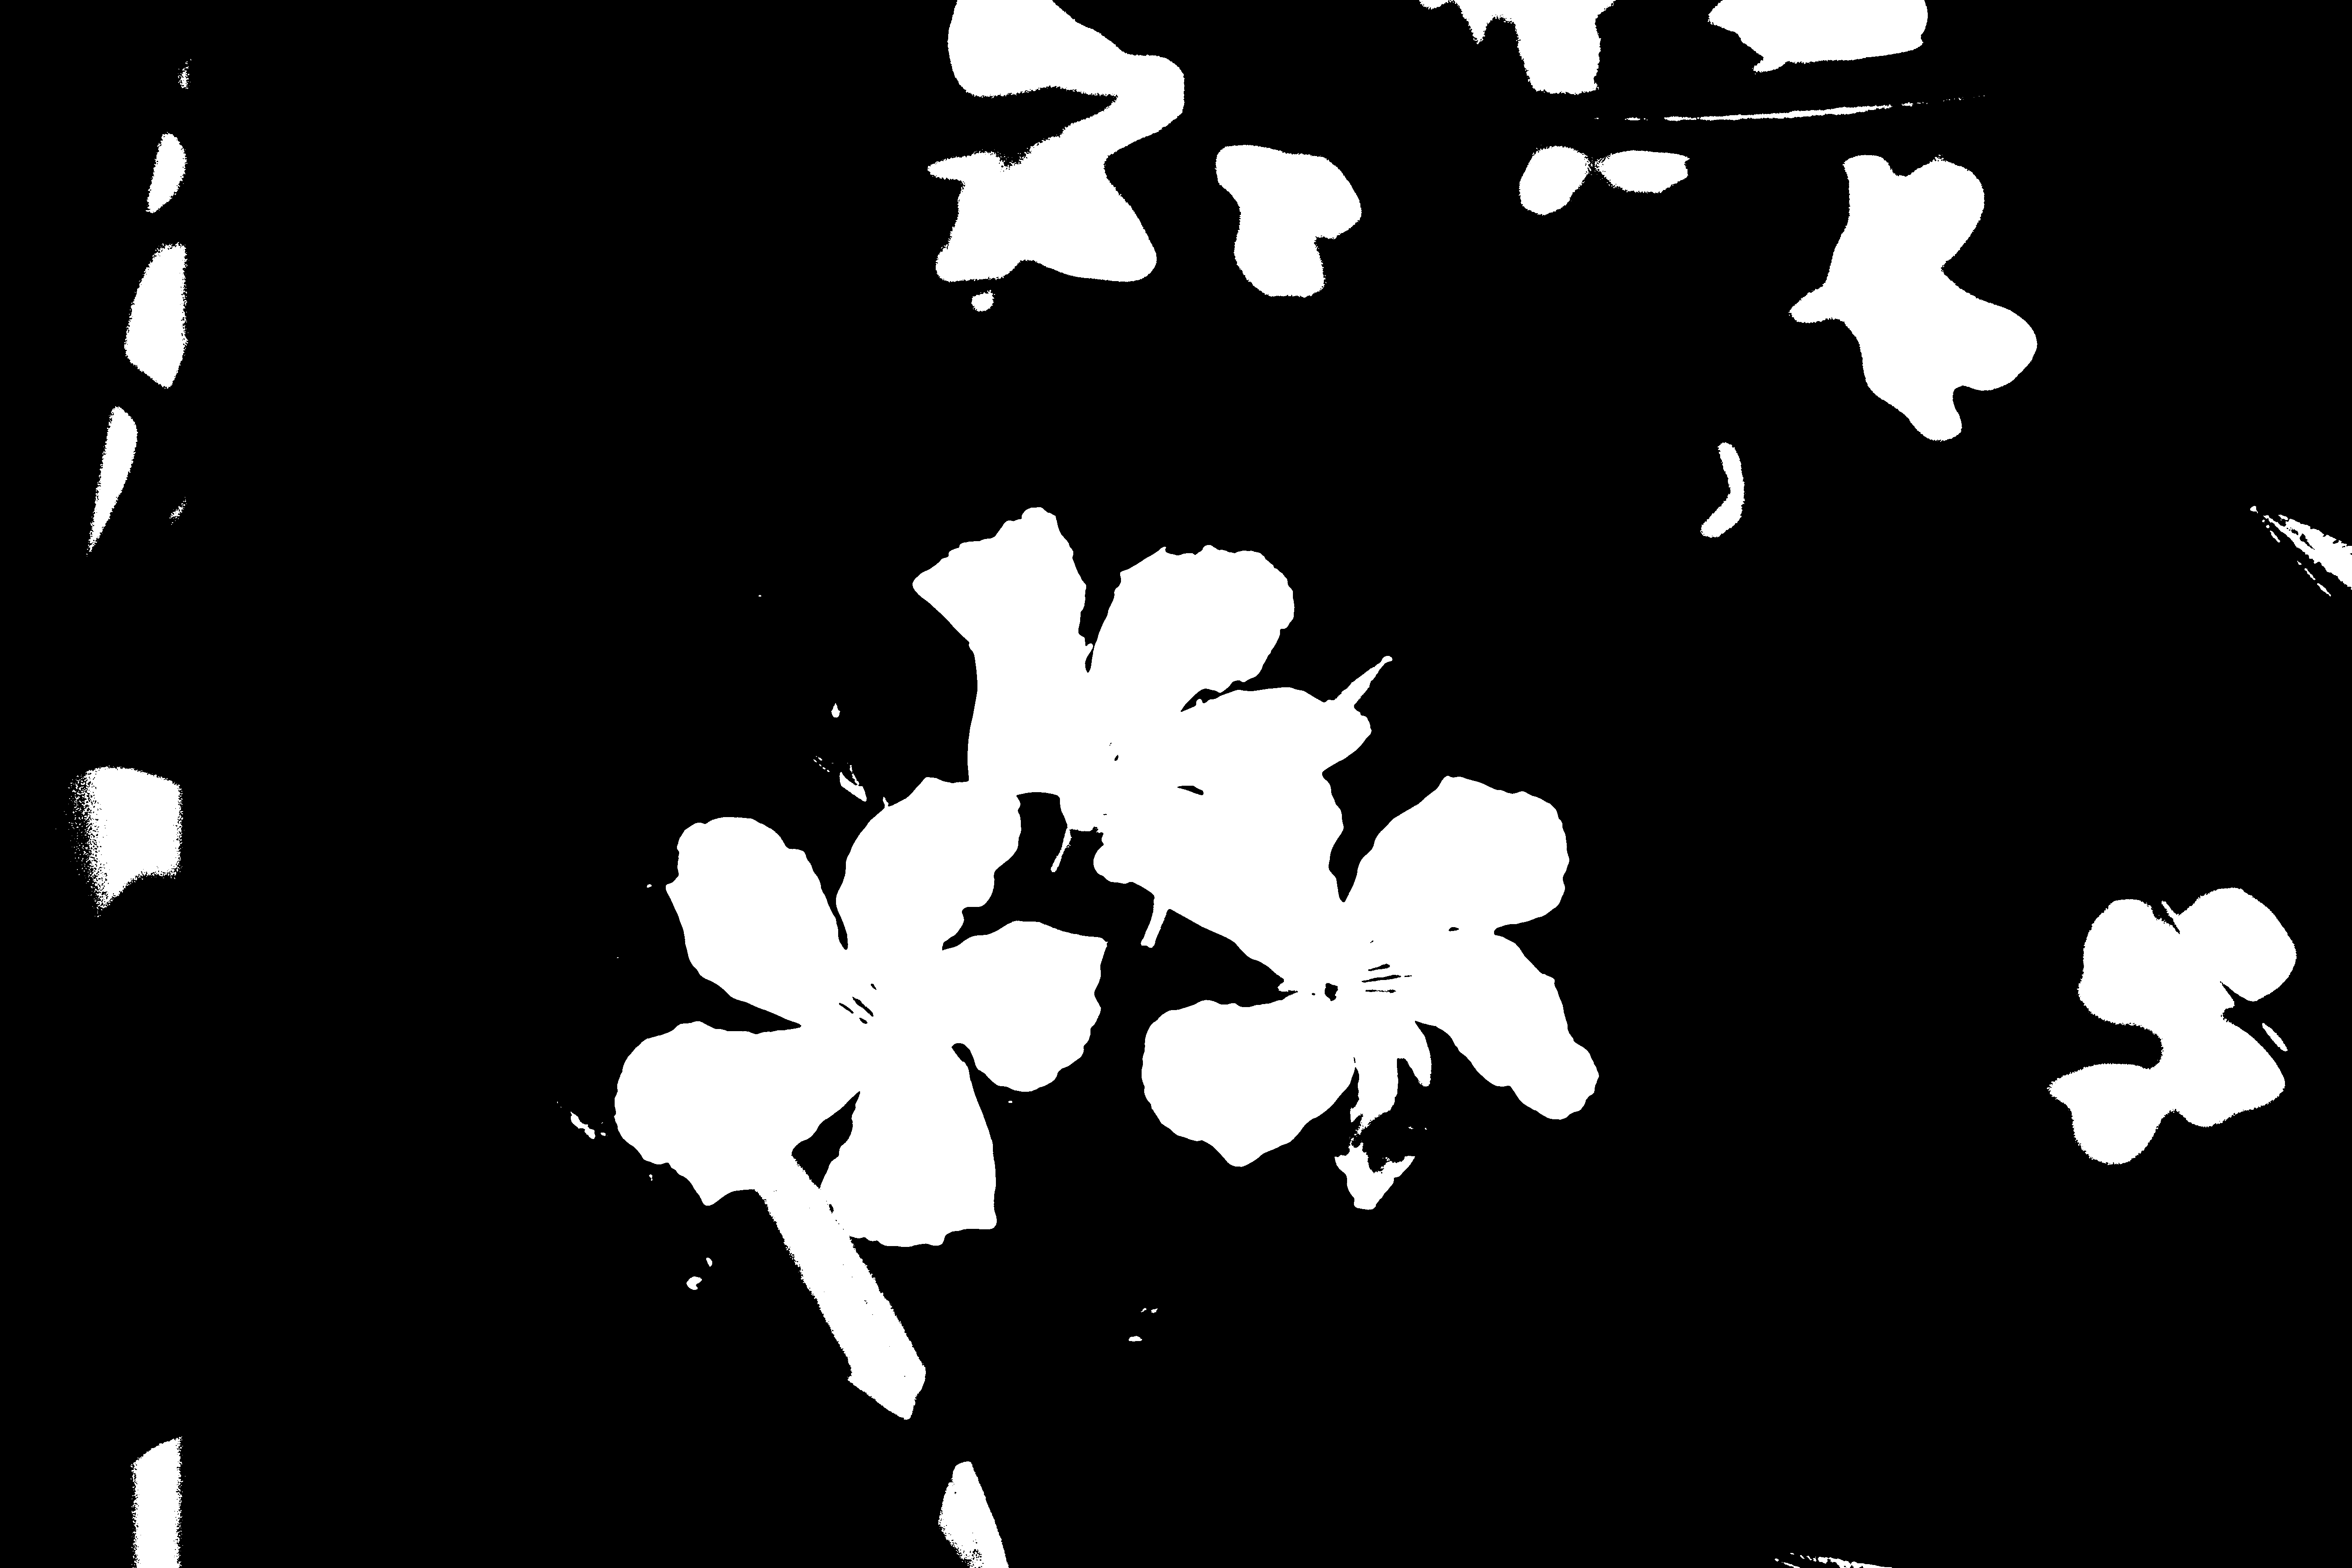
\includegraphics[scale=0.04]{A3_thresh.png} \\ \\

We managed to get the flowers by applying thresholding. After this step, we need to remove the background artifacts. To be able to do this, we need to apply morphological operations to the image. We decided to choose the kernel size as (5,5). \\ \\

First, we erode our image with cv.erode function and secondly, we use cv.dilate function to preserve our flower size. \\

After applying morphological operations and converting our flowers into white color, we had an image like this: \\ \\
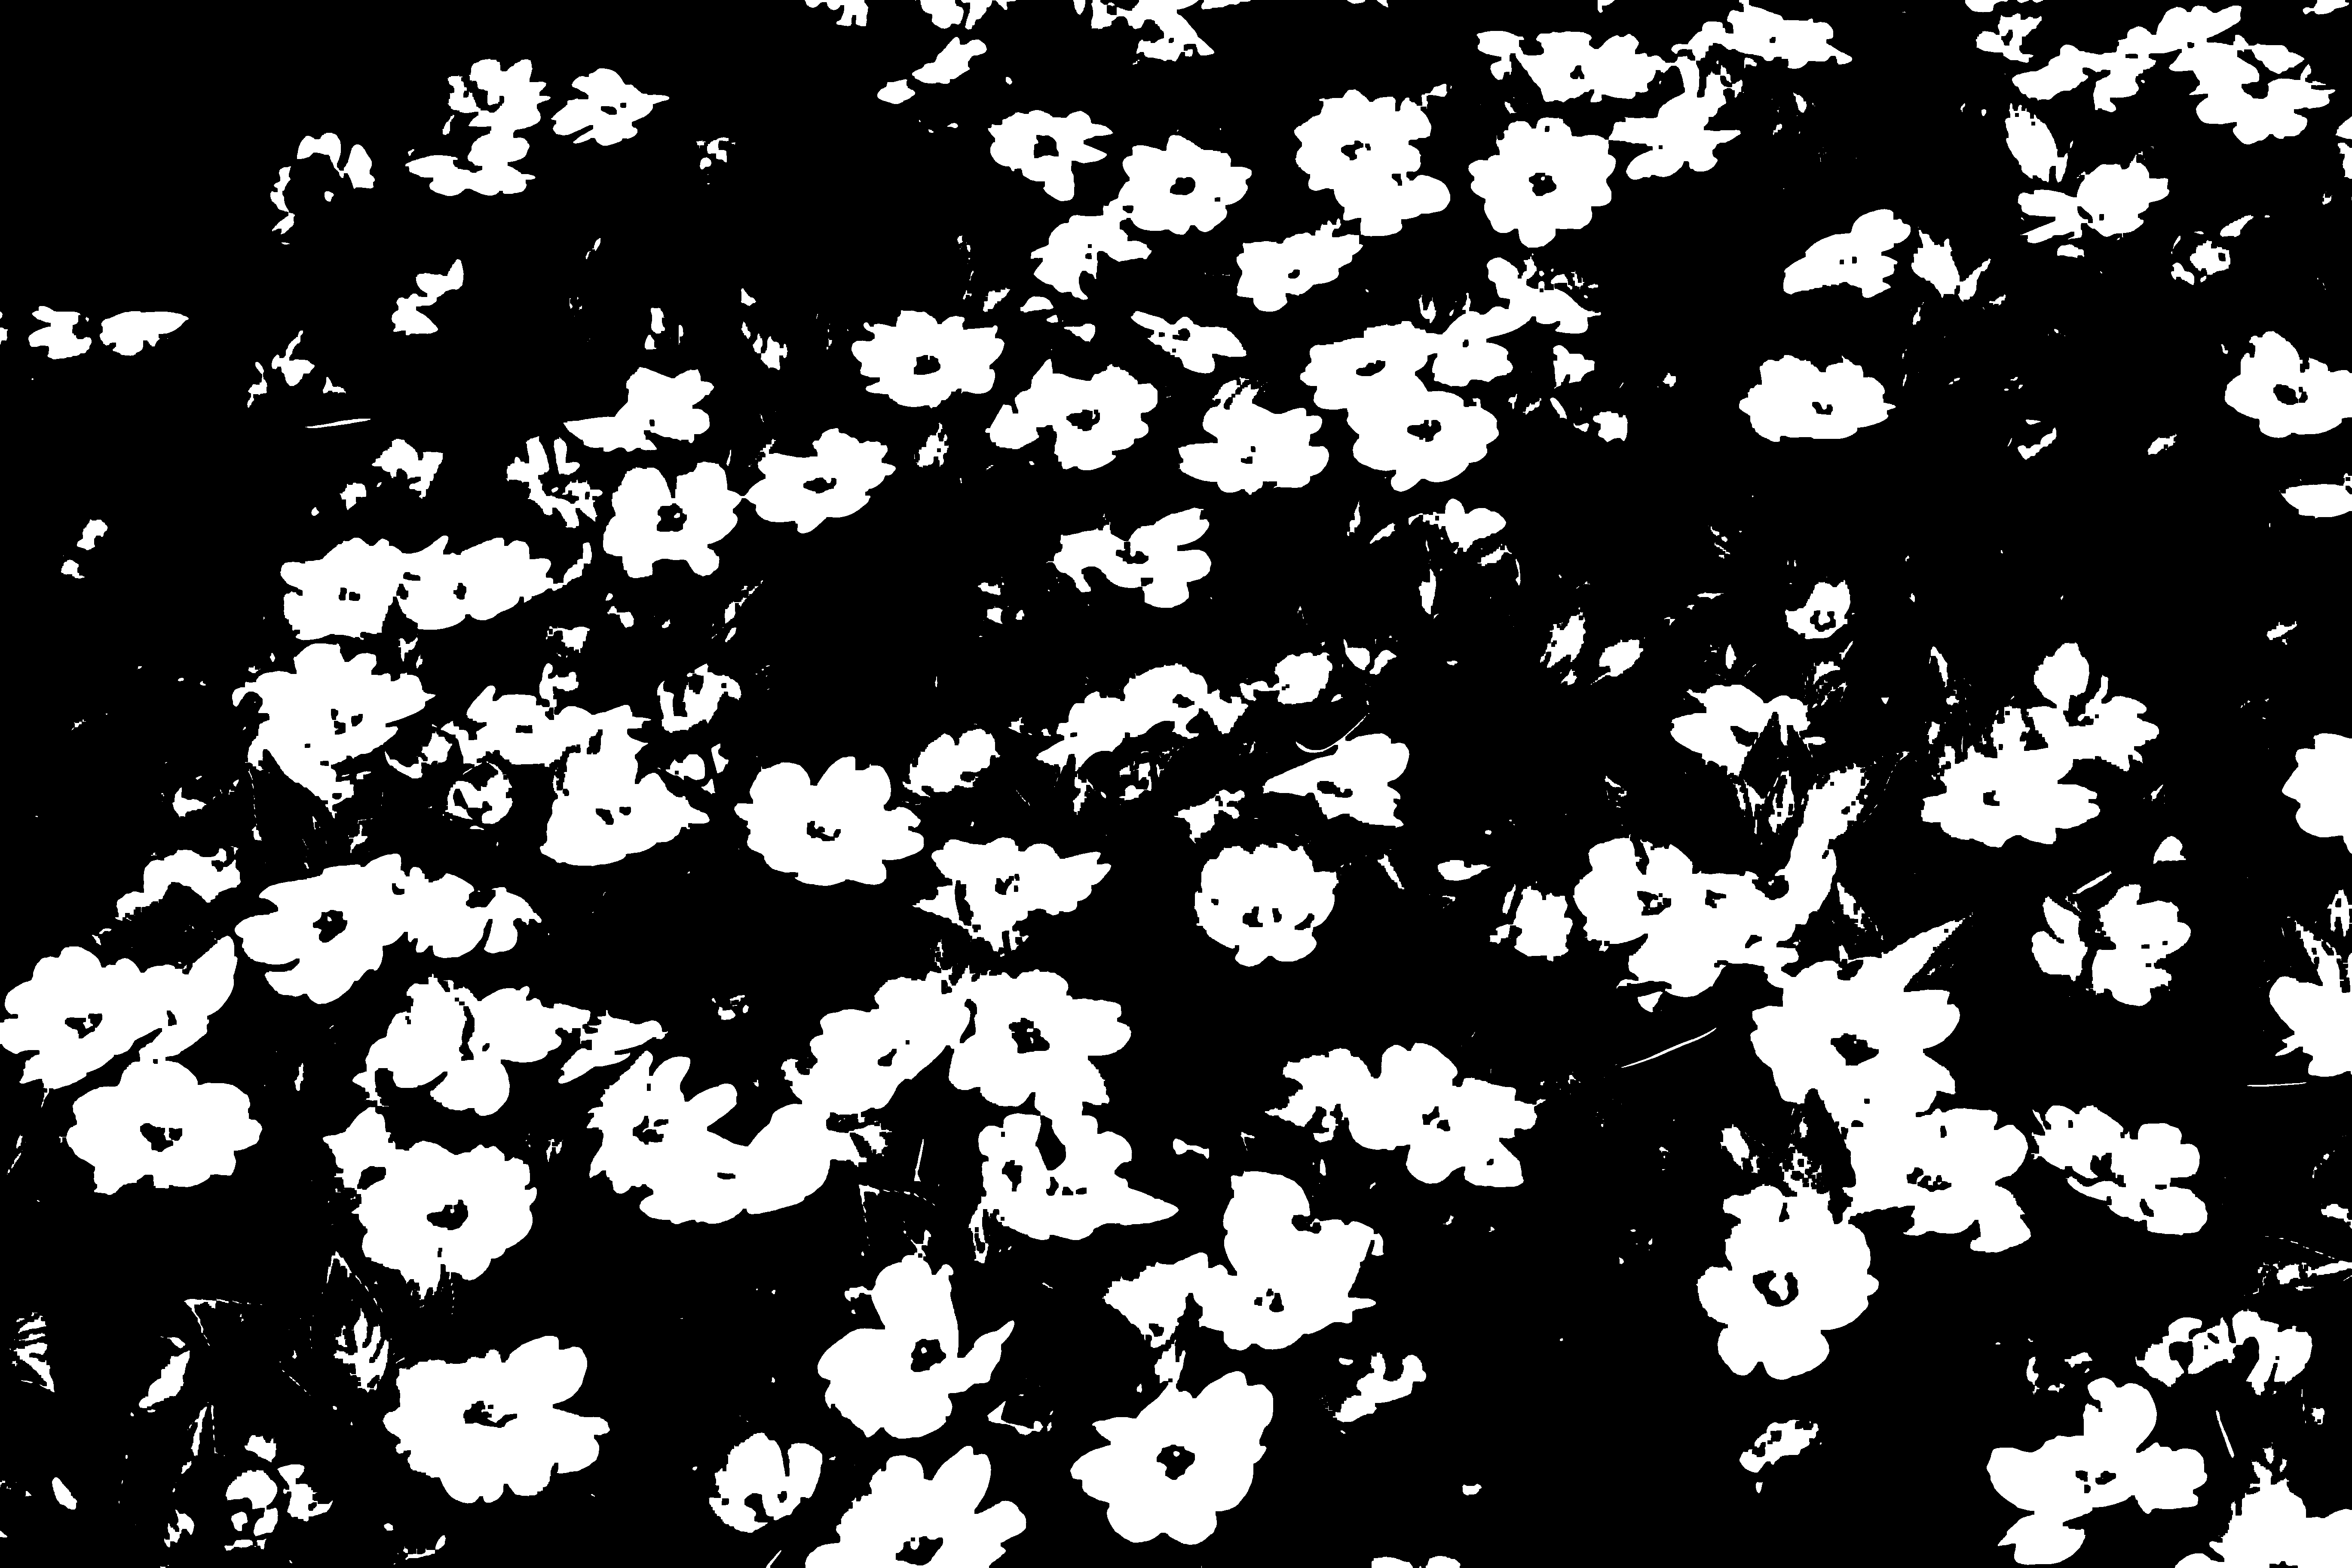
\includegraphics[scale=0.04]{A1.png} \\ \\
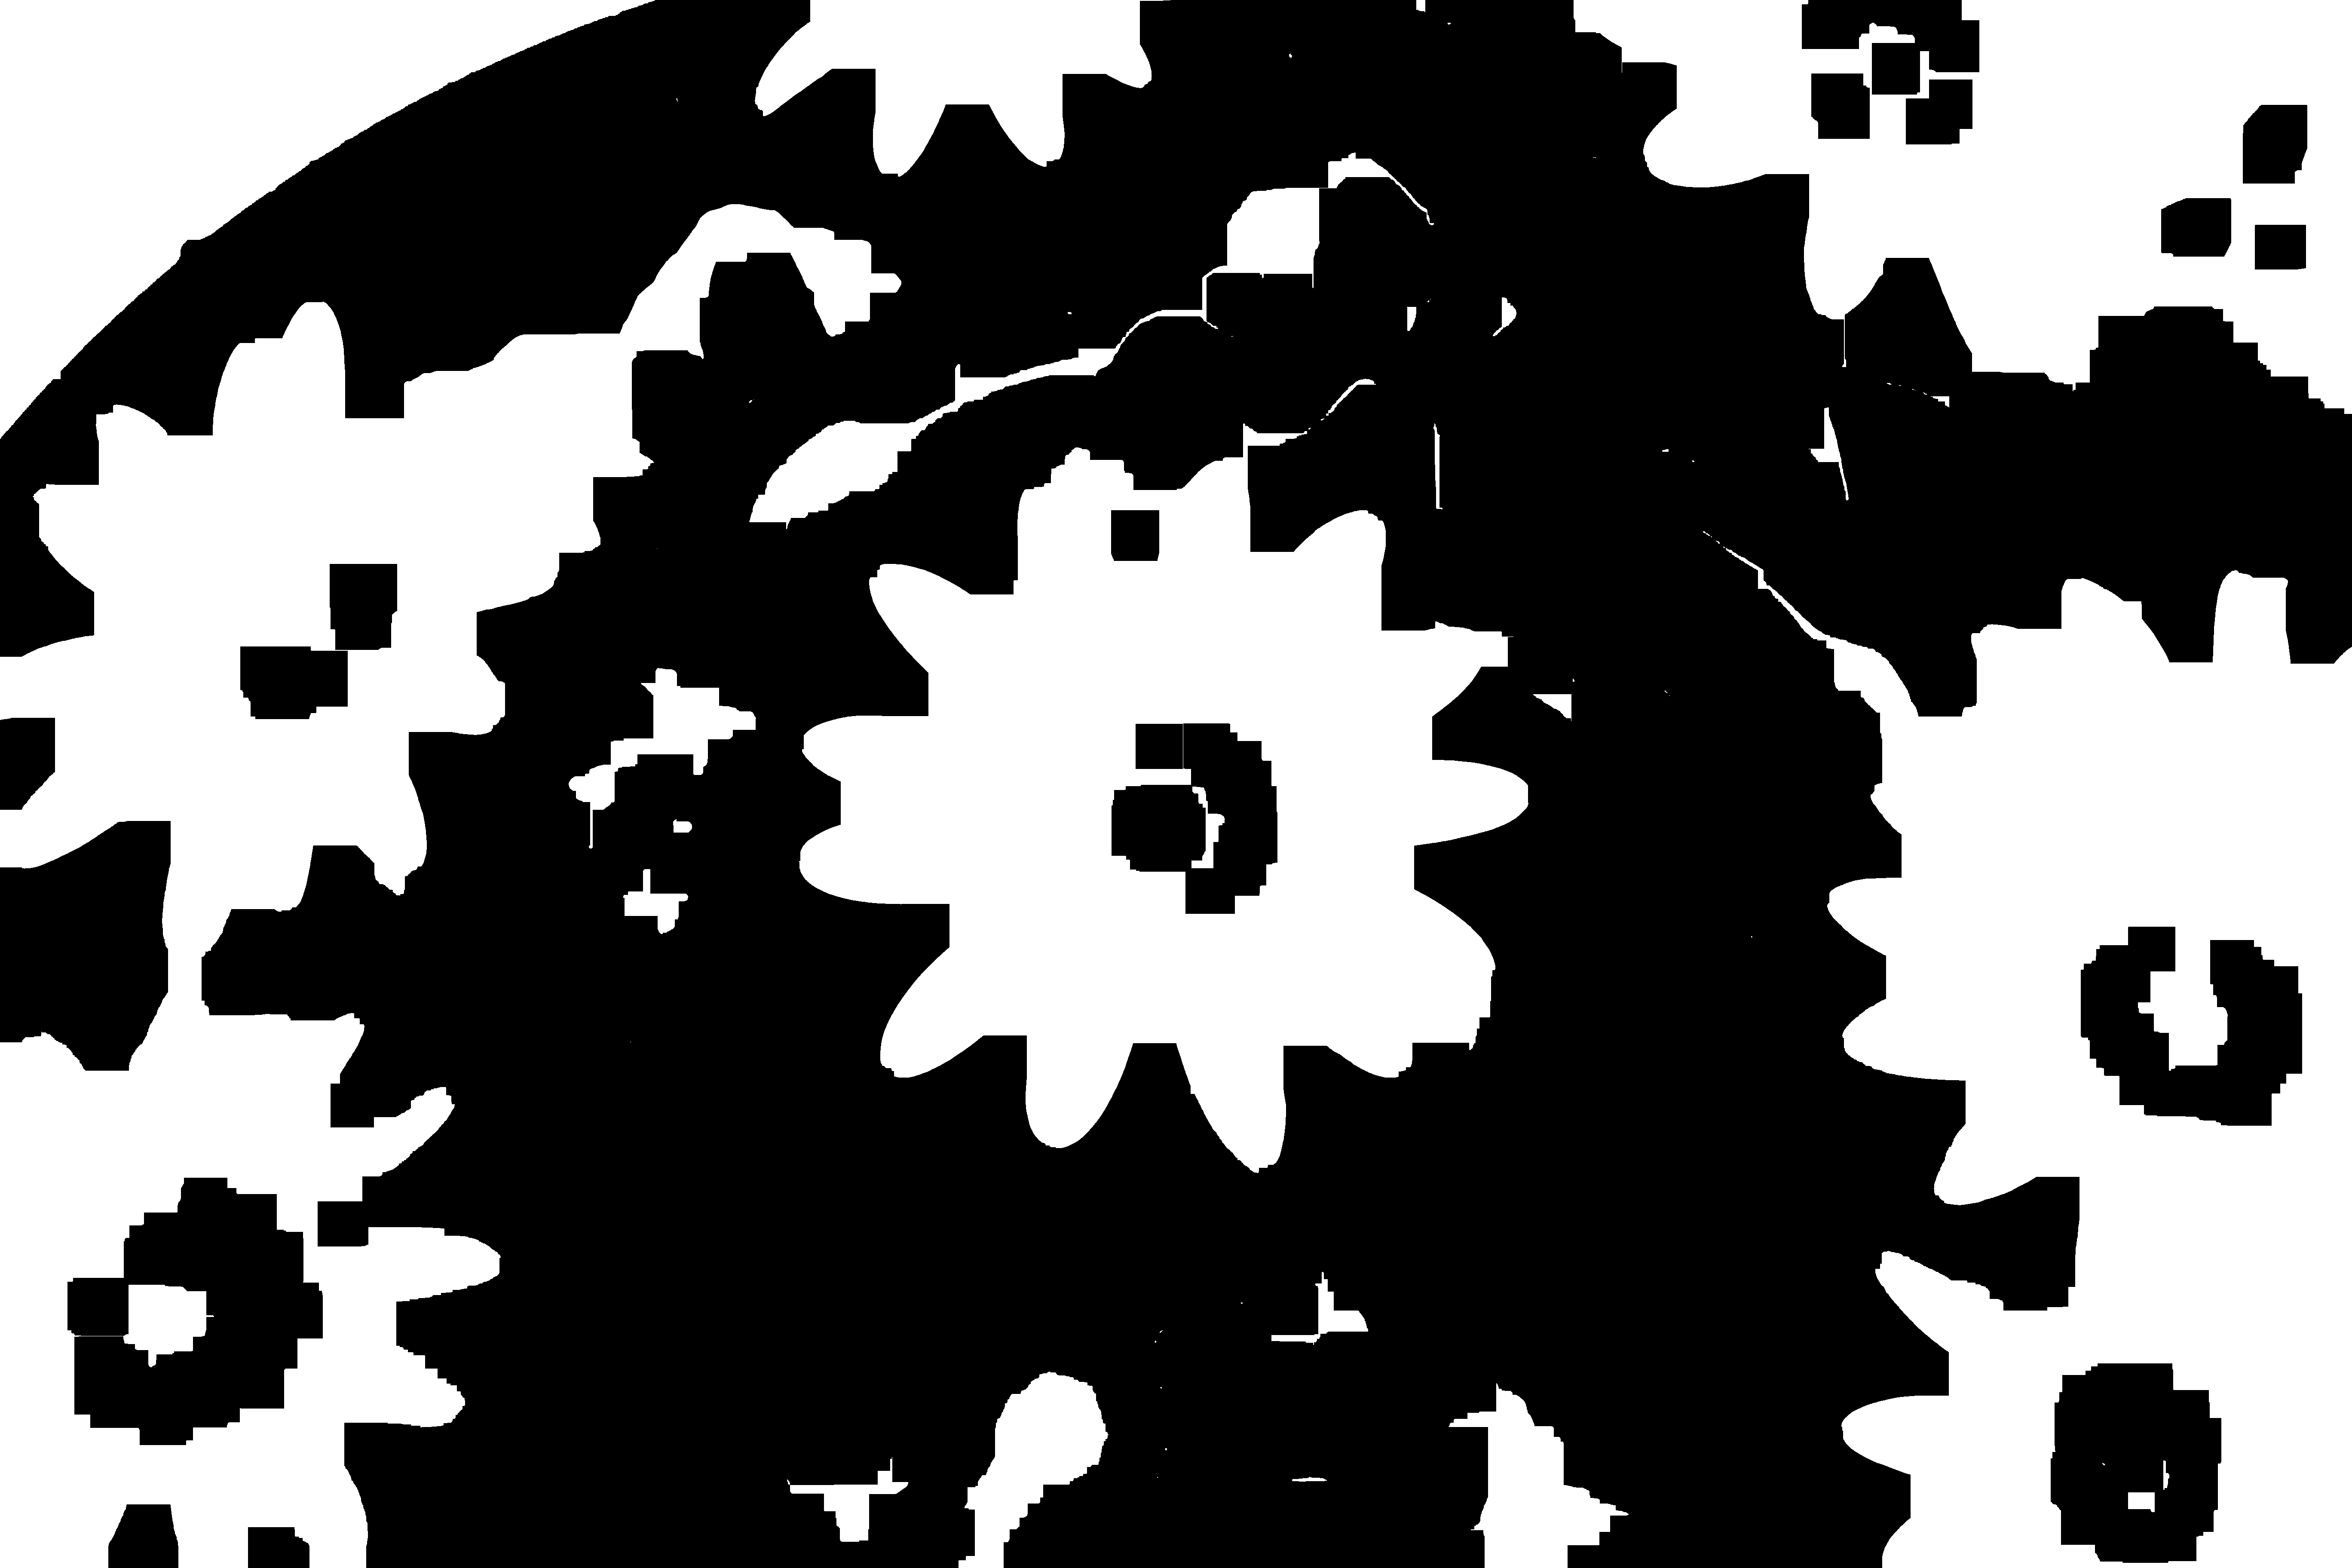
\includegraphics[scale=0.04]{A2.png} \\ \\
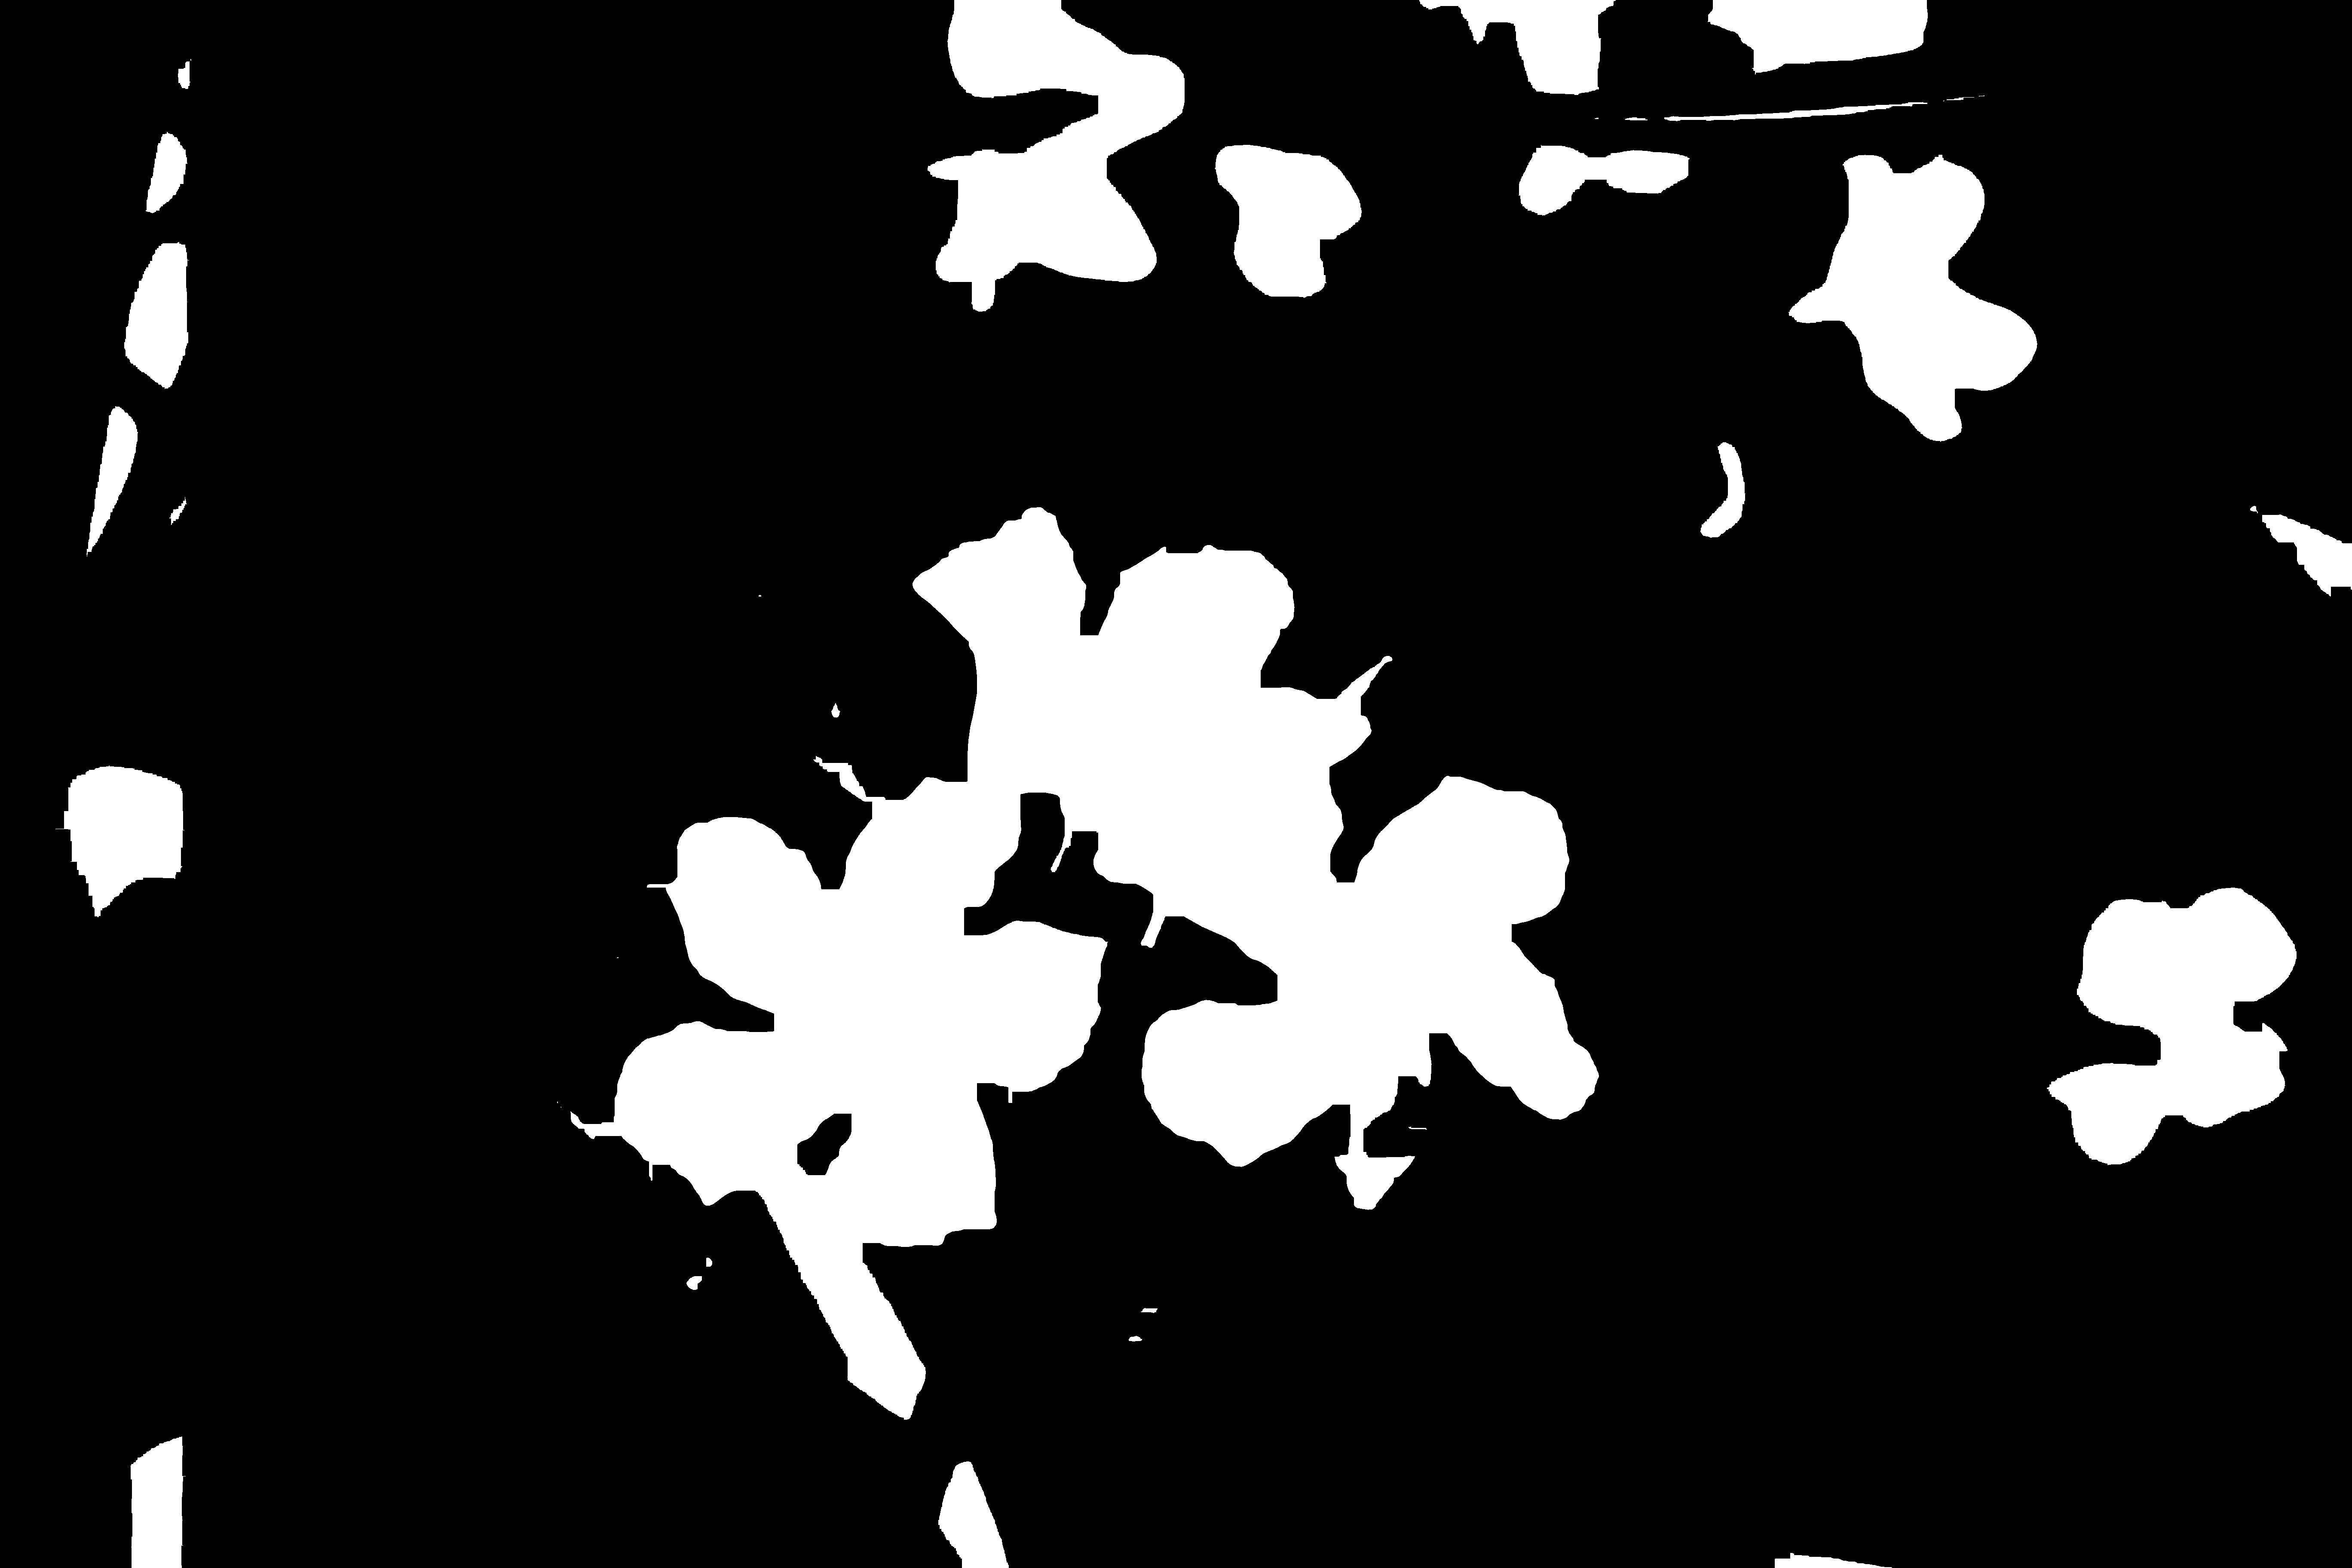
\includegraphics[scale=0.04]{A3.png} \\ \\

We are able to get rid of most of the background artifacts and now we need to do one last thing to find the count of flowers: Counting the closed regions.

To count the closed regions, we used cv.findContours function. This function gives us the connected and closed regions. We used this function but we have a problem now: We are trying to find the number of flowers but there are also background artifacts in our image. So, we need to eliminate some regions. \\

To eliminate the background artifacts, we decided to average areas of all regions and eliminate the regions with areas below the $average*0.4$. \\

Lastly, we can find the number of flowers by counting the number of contours.

\section{Segmentation}
In this part, we created two parameter sets for n-cut and mean shift segmentation types.\\

For n-cut segmentation, we use compactness, n\_segments, and max\_num\_iter parameters. Compactness is given to segmentation.slic method of skimage library. It basically makes superpixel shapes more clear, like square or cubic shapes. n\_segments is also given to segmentation.slic method, which is an approximation to the number of labels. max\_num\_iter is another parameter, which is used for the number of iterations we expect from the algorithm. \\

For mean shift segmentation, we created quantile, n\_samples, and max\_iter attributes. quantity parameter decides which part of pairwise distances should be used. It is given as 0.3 by default. n\_samples determines the number of samples to be used, and max\_iter is the same as in the n-cut parameters.\\

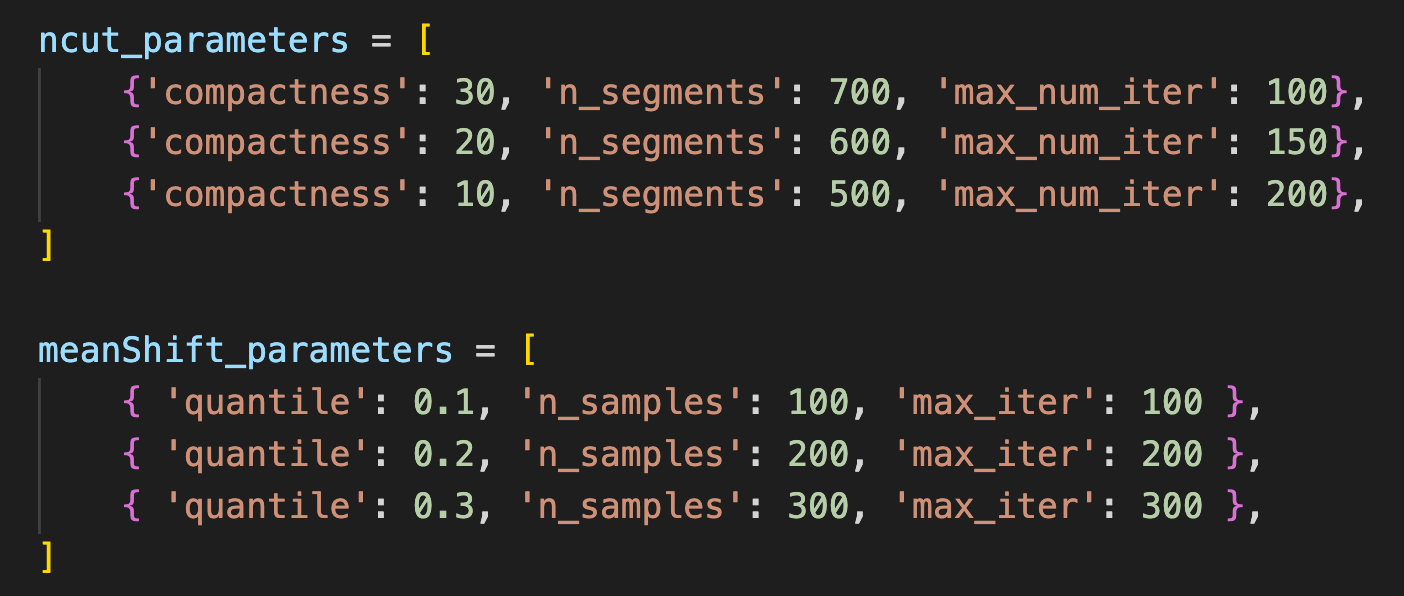
\includegraphics[width=0.9\linewidth]{parameters.png}
\\
\textit{Parameter sets for n-cut and Mean Shift segmentations}\\

\subsection{Method}

We call makeSegmentation() function from the main function. In makeSegmentation, we basically call segmentationFn function with all parameters, all images, and all algorithms.\\

segmentationFn blurs the image by cv.blur method, in order to reduce unnecessary details in the image. Then it calls segmentation method, which is ncut, or meanShift, regarding to the selected algorithm. meanShift method flattens the image to one dimension and estimates the bandwidth according to the given parameters to estimate\_bandwidth function. With the obtained bandwidth, we call cluster.MeanShift function of sklearn library, then fit it to our image. This method gives us labels and centers. We fill all of the pixels with given labels and centers, basically we map a center to all of the pixels and label this center. Then we create image by this information.\\

For n-cut segmentation, we create ncut function. It extracts labels by calling segmentation.slic function with the given parameters. Then we create a rag and apply cutting to the result. We fill the image with color by applying labels2 to the pixels, and return the output.\\

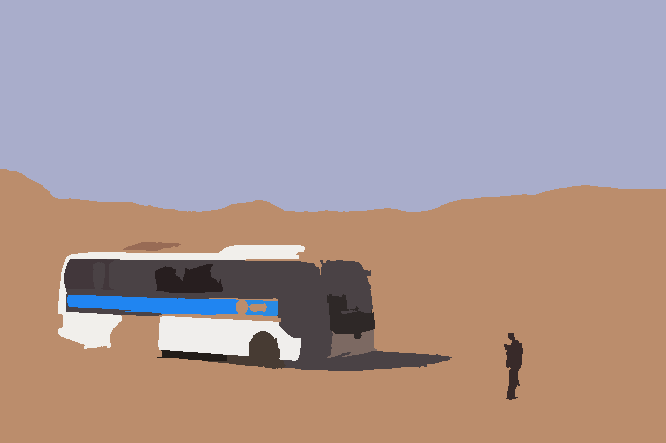
\includegraphics[width=0.9\linewidth]{segment.png}
\\
\textit{n-cut segmentation result for B3.png with parameter set 3}\\

After having segmented image, we blur it further and extract edges by canny edge detector, using cv.Canny method of OpenCv2 library. Then we apply thresholding and morphology to the edges, in order to reduce the number of segments, and create clearer graphs. One of the return values of cv.findContours is hierarchy, which denotes all of the segments and its parent-child relationships. With this information, creating DAG and tree relationship structure is simple.\\

We created a helper method for tree relationship structure, which creates a Graph from networkx library. We basically add edges between parents and childs regarding to the information obtained by hierarchy. Then we save this image with matplotlib savefig method to use in the future.\\

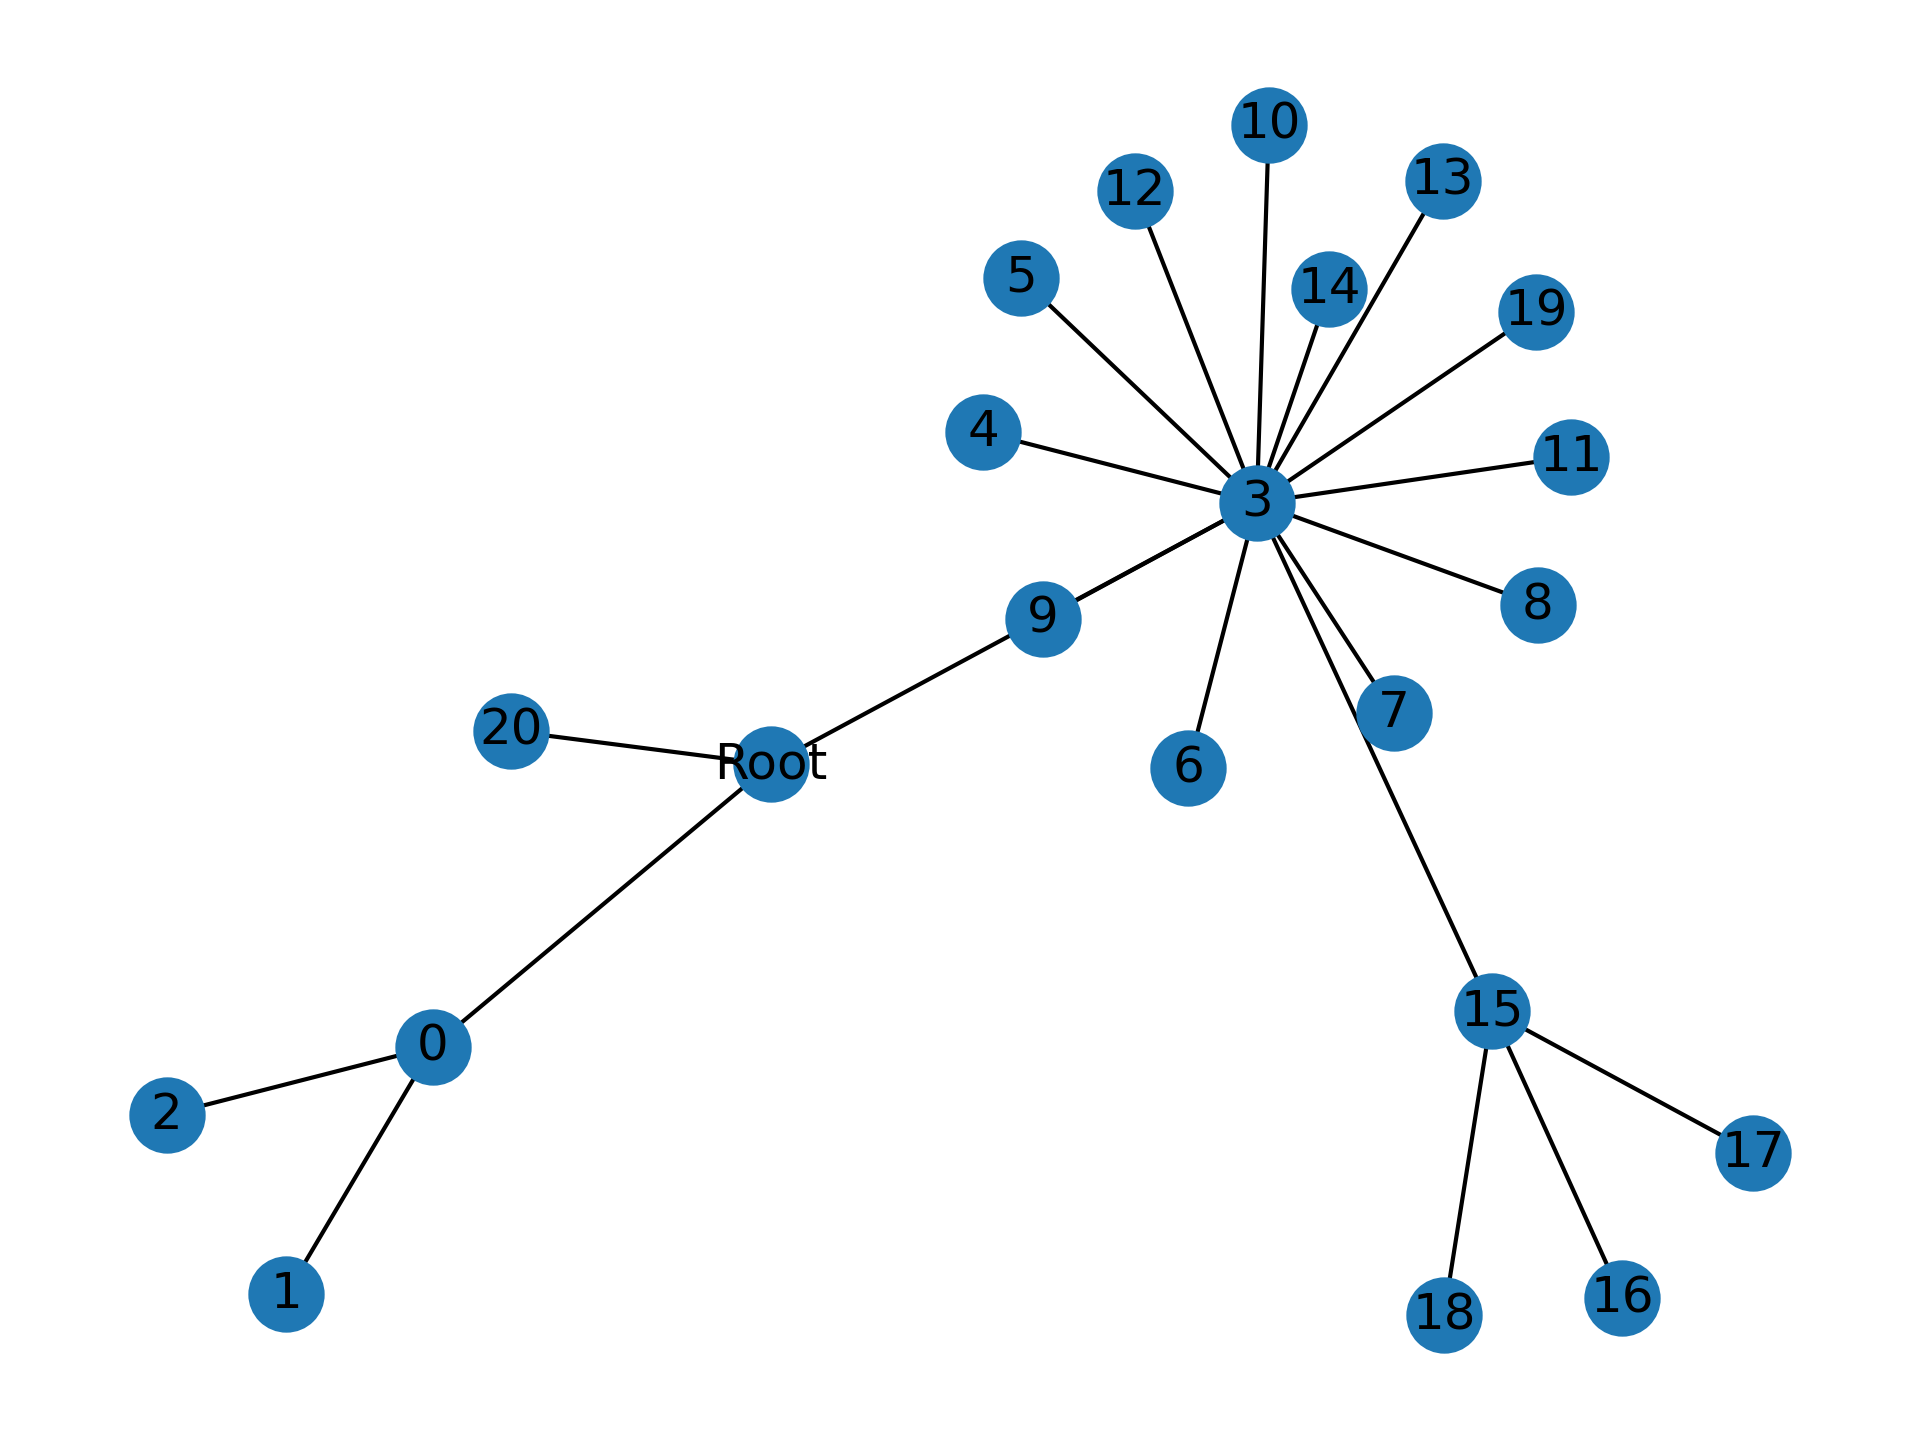
\includegraphics[width=0.9\linewidth]{tree.png}
\\
\textit{Tree relationship structure for n-cut segmented image of B3.png with parameter set 3}\\


Finding region adjacency graph is possible by looking at the values of hierarchy. We created a graph.rag.RAG structure from skimage.future library. We drew this RAG with networkx library and saved the result to use in the future.\\

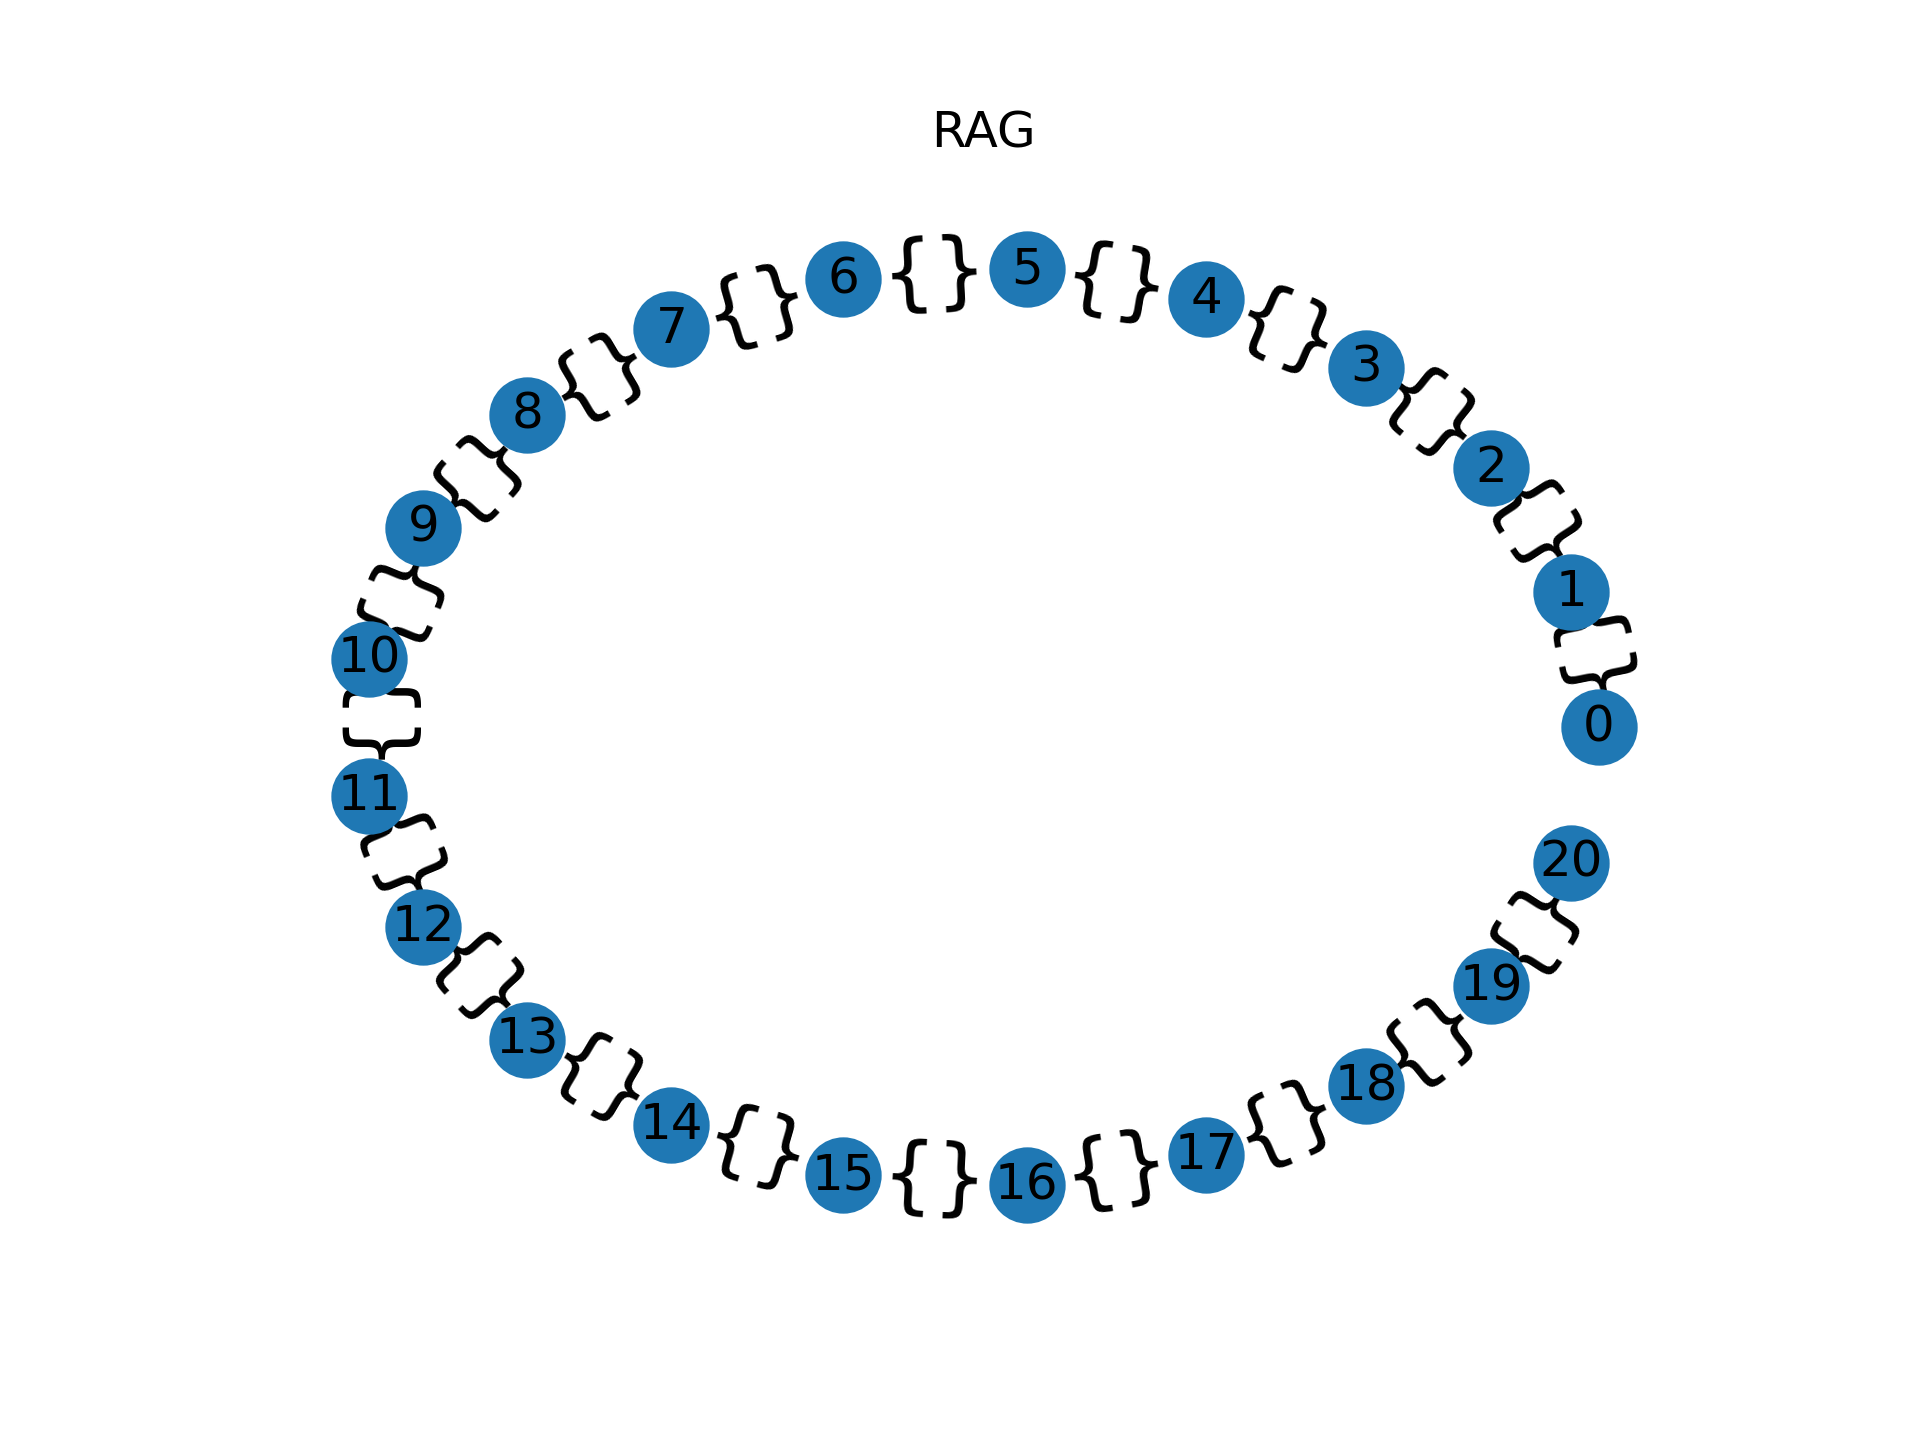
\includegraphics[width=0.9\linewidth]{rag.png}
\\
\textit{RAG for n-cut segmented image of B3.png with parameter set 3}\\


Drawing boundary overlay is possible by looking at the result obtained from canny edge detector. We basically copy the original image to a new image, and fill the pixels where edge result is 255 by green color.\\

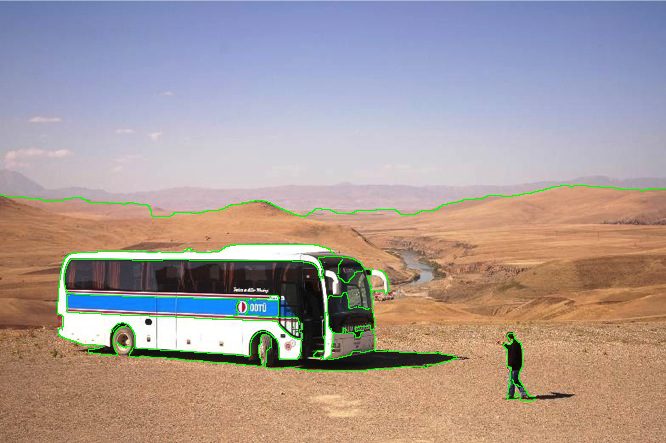
\includegraphics[width=0.9\linewidth]{boundary.png}
\\
\textit{Boundary overlay for n-cut segmented image of B3.png with parameter set 3}\\

Then we concatenate the images by np.concatenate function and save the image to Outputs folder.

\newpage

\onecolumn
\subsection{Results}

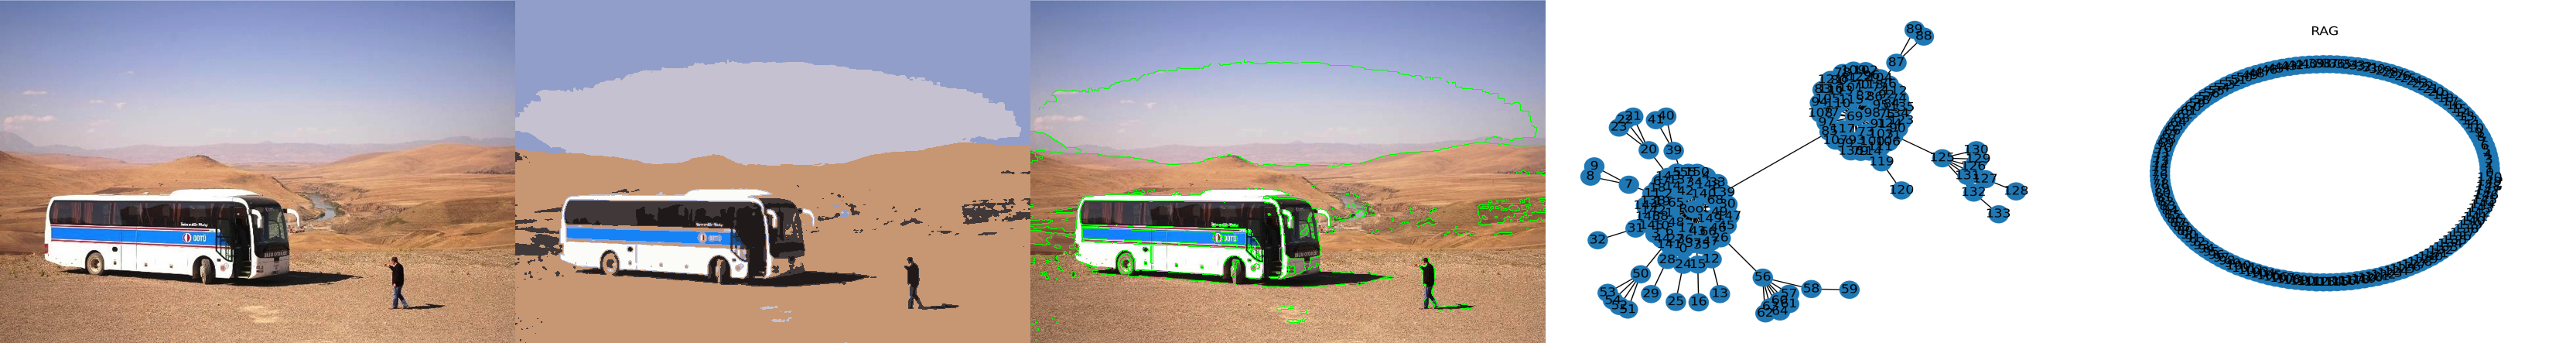
\includegraphics[width=0.9\linewidth]{B3_algorithm_meanshift_parameterset_1.png}
\\
\textit{Result of B3.png with mean shift segmentation and parameter set 1}\\

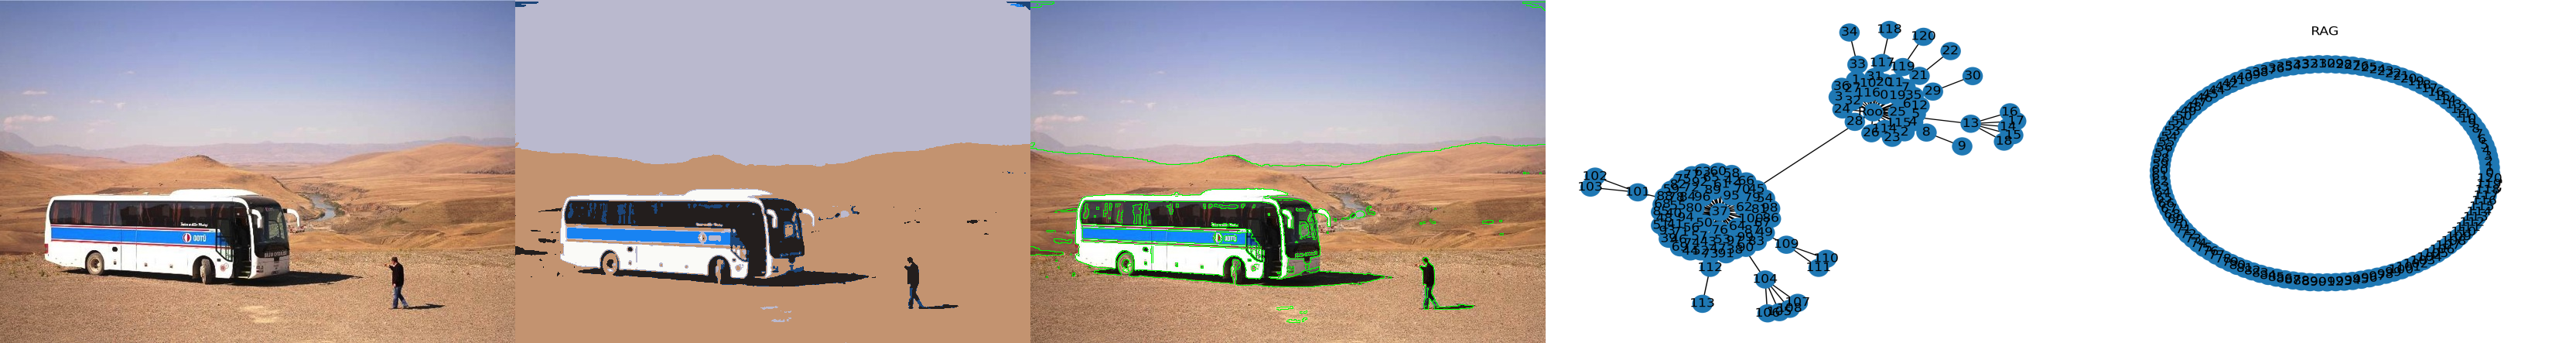
\includegraphics[width=0.9\linewidth]{B3_algorithm_meanshift_parameterset_2.png}
\\
\textit{Result of B3.png with mean shift segmentation and parameter set 2}\\

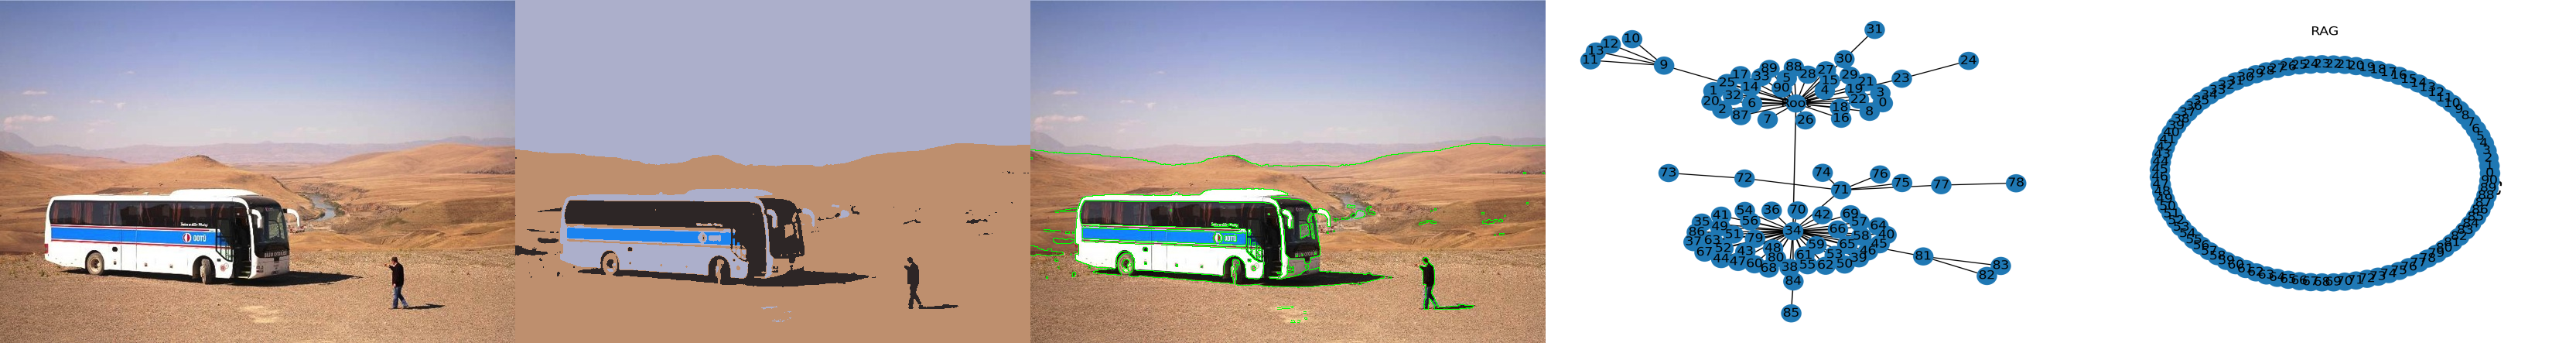
\includegraphics[width=0.9\linewidth]{B3_algorithm_meanshift_parameterset_3.png}
\\
\textit{Result of B3.png with mean shift segmentation and parameter set 3}\\

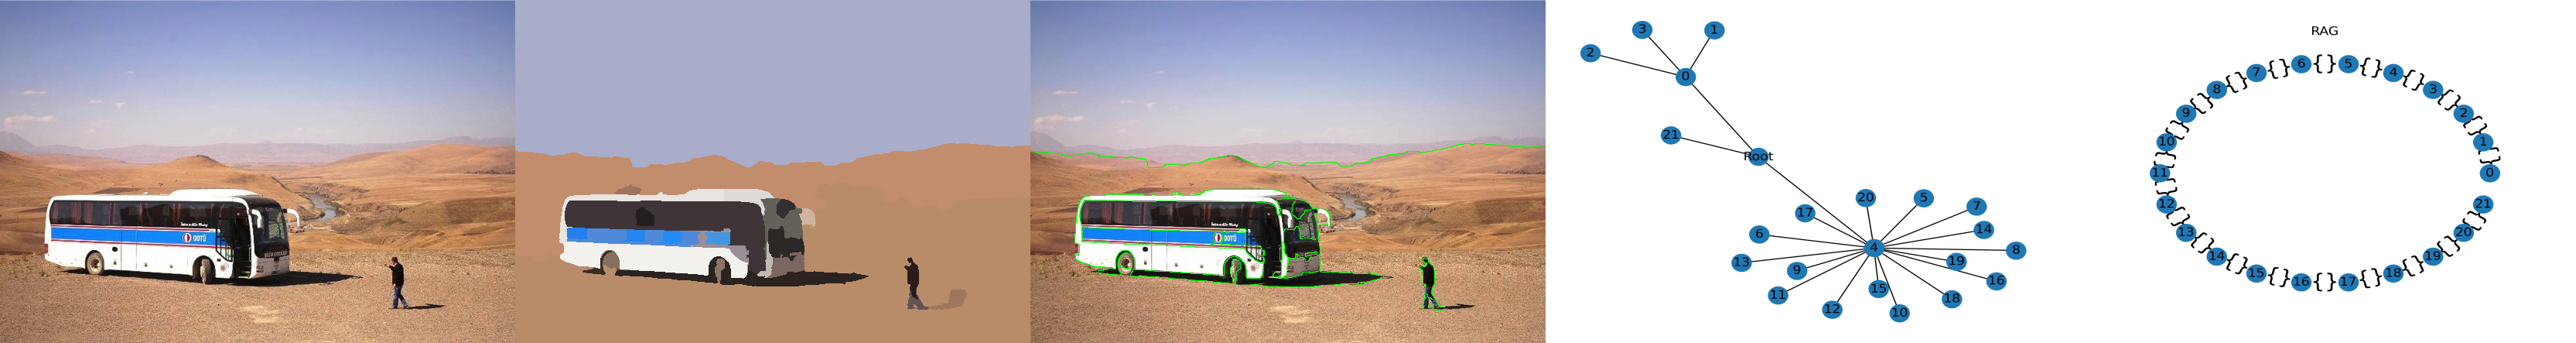
\includegraphics[width=0.9\linewidth]{B3_algorithm_ncut_parameterset_1.png}
\\
\textit{Result of B3.png with n-cut segmentation and parameter set 1}\\

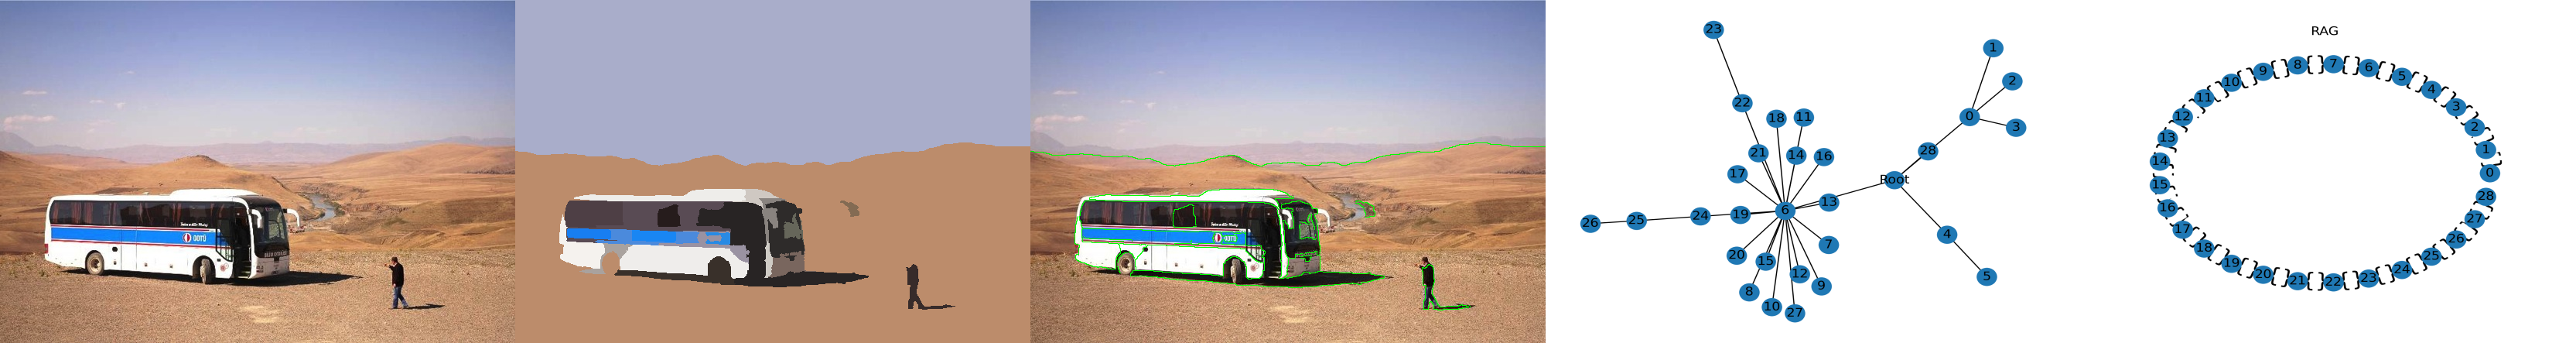
\includegraphics[width=0.9\linewidth]{B3_algorithm_ncut_parameterset_2.png}
\\
\textit{Result of B3.png with n-cut segmentation and parameter set 2}\\

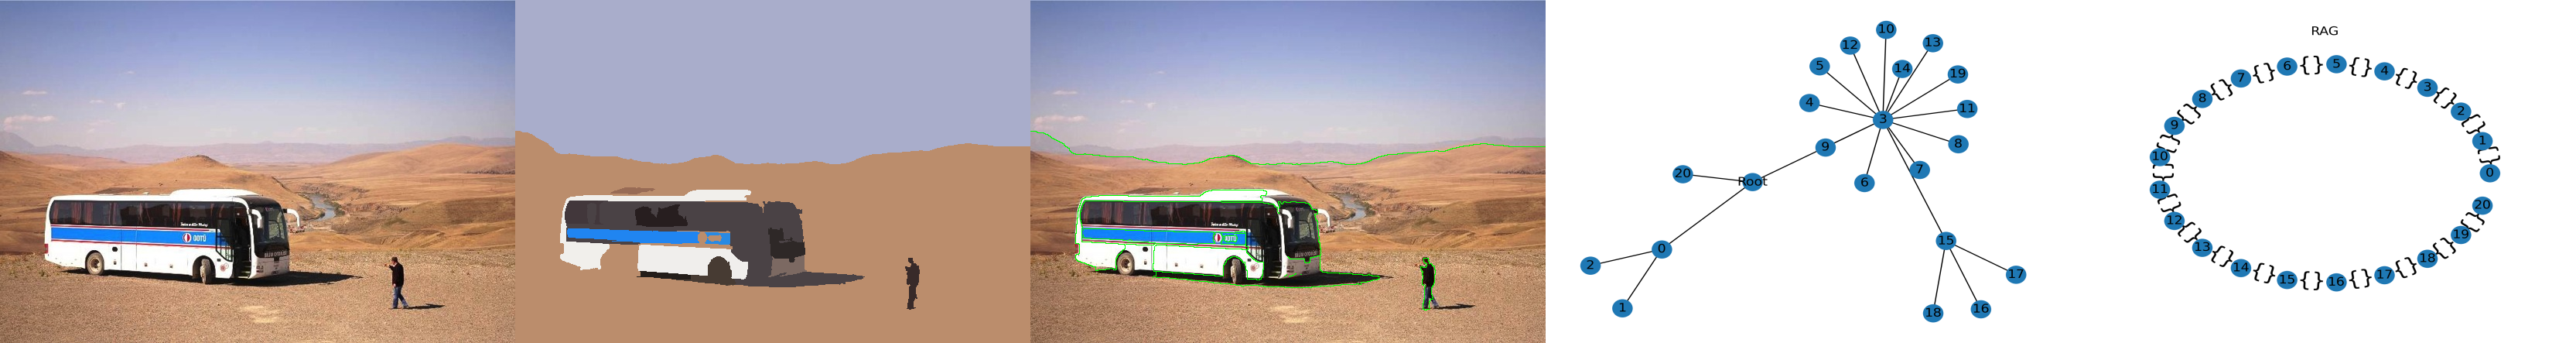
\includegraphics[width=0.9\linewidth]{B3_algorithm_ncut_parameterset_3.png}
\\
\textit{Result of B3.png with n-cut segmentation and parameter set 3}\\

Mean shift segmentation created a lot of segments related to the image, and it is usually not desired. We tried different parameter sets and different pre-processing methods to decrease the number of segments, but it created way more segments than expected. It may be used to obtain sensitive information about the image, but this time, RAG and tree relationship structure will be more complicated.

N-cut segmentation is ideal for extracting smoother results. It also works faster than mean shift segmentation. This result may be misleading as we used different methods and different libraries, but for this homework, the results obtained from n-cut segmentation is way more simpler and clearer than mean shift segmentation. 
\end{document}
